%\svnInfo $Id: Ch2_2017.tex 67 2017-09-12 08:21:29Z Georg Lindgren $  
%$
%
\chapter{Random waves and loads}
\label{cha:rand-loads-stoch}\label{cha:2}

In this chapter we present some tools for analysis of random functions
with respect to their correlation, spectral, and distributional
properties. We first give a brief introduction to the theory of Gaussian
processes and then we present programs in \progname{},
which can be used to analyse random functions. For deeper insight in the theory 
we refer to \cite{Lindgren2013,LindgrenRootzenSandsten2014}.

The presentation will be organized in three examples:
Example~\ref{Ex_sea_statistics}
is devoted to estimation of different parameters in the model,
Example~\ref{Ex_sea_spectra}
deals with spectral densities and
Example~\ref{Ex_sea_simulation}
presents the use of \progname{} to simulate samples of a Gaussian process.
The commands, collected in \verb+Chapter2.m+, run in less than
5~seconds on a 3.60~GHz 64 bit PC with Windows 10; add another two minutes 
for the display of simulated wave fields.

\section{Introduction and preliminary analysis}
\label{sec:intr-prel-analys}\label{sect2.1}
The functions we shall analyse can be measured stresses or strains,
which we call loads, or other measurements, where waves on the sea
surface is one of the most important examples.
We assume that the measured data are given in one of the following  forms:

\begin{enumerate}
\item In the time domain, as measurements of a response function
denoted by $x(t)$, $0\le t\le T$, where $t$ is time and $T$ is the
duration of the measurements. The  $x(t)$-function is usually
sampled with a fixed sampling frequency and a given resolution,
i.e.\ the values of $x(t)$ are also discretised. The effects of
sampling can not always be neglected in estimation of parameters
or distributions. We assume that measured functions are saved as a
two column ASCII or {\tt mat} file.

Some general properties of measured functions can be
summarized by using a few simple characteristics. Those are the
\emph{mean} $m$, defined as the average of all values, the
\emph{standard deviation} $\sigma$, and the \emph{variance}
$\sigma^2$, which measure the variability around the mean in linear
and quadratic scale. These quantities are estimated by
\begin{eqnarray}
m &=&1/T\,\int_0^T x(t)\, \rd t, \\
\sigma^2 &=& 1/T\,\int_0^T (x(t)-m)^2\, \rd t,
\end{eqnarray}
for a continuous recording or by corresponding sums for a sampled series.

\item In the frequency domain, as a power spectrum, which is an
important mode in systems analysis. This means that the signal
is represented by a Fourier series,
\begin{equation}
x(t)\approx
m + \sum_{i=1}^N a_i\cos(\omega_i\,t)+b_i
\sin(\omega_i\,t),
\label{eqn:fourier_series}
\end{equation}
where $\omega_i=i\cdot 2\pi/T$ are angular
frequencies,
$m$ is the mean of the signal and $a_i,b_i$ are Fourier coefficients.

\item Another important way to represent a load sequence is by means of
the \emph{crossing spectrum}\index[xentr]{crossing spectrum}
\index[xentr]{spectrum!crossing} or
\emph{ crossing intensity},
\index[xentr]{crossing intensity}
$\mu(u)$ = the intensity of
upcrossings = average number of upcrossings per time unit, of a
level $u$ by $x(t)$ as a function of $u$,
see further in Section~\ref{subsec:crossing_intensity}.
The \emph{mean frequency}\index[xentr]{mean frequency}
$f_0$ is usually defined as the number of
times $x(t)$ crosses upwards (upcrosses) the mean level  $m$
normalized by the length of the observation interval $T$, i.e.\
$f_0=\mu(m)$. An alternative definition,\footnote{Still another
  definition, to be used in Chapter~\ref{cha:5},
is that $f_0$ is the average number of completed load cycles per time
unit.} which we prefer to use is that $f_0=\max \mu(u))$, i.e.
it is equal to the maximum of $\mu(u)$.
The \emph{irregularity factor}\index[xentr]{irregularity factor}
$\alpha$ is defined as the mean frequency $f_0$
divided by the intensity of local maxima (``intensity of cycles'', i.e.\
the average number of local maxima per time unit)
in $x(t)$. Note, a small $\alpha$ means an irregular process,
$0 < \alpha \leq 1$.
\end{enumerate}

\begin{rtex}{Ex_sea_statistics}{Sea data}\label{pageseadat}
In this example we use a series with wave data {\tt sea.dat}
with time argument in the first column and function values in
the second column. The data used in the examples are wave measurements
at shallow water location, sampled with a sampling frequency
of~4~Hz, and the units of measurement are seconds and meters, respectively.
The file {\tt sea.dat} is loaded into \ML{} and after the mean
value has been subtracted the data are saved in the two column matrix
{\tt xx}.
{\small\begin{verbatim}
      xx = load('sea.dat');
      me = mean(xx(:,2))
      sa = std(xx(:,2))
      xx(:,2) = xx(:,2) - me;
      lc = dat2lc(xx);
      plotflag = 2;
      lcplot(lc,plotflag,0,sa)
\end{verbatim}}\index[xcmds]{{\tt dat2lc}}\index[xcmds]{{\tt lcplot}}
Here {\tt me} and {\tt sa} are the mean and standard deviation of the signal,
respectively. The variable {\tt lc} is a two column matrix with
levels in the first column and the number of upcrossing of the level in
the second. In Figure~\ref{fig1_cr} the number of upcrossings of
{\tt xx} is plotted and compared with an estimation based on the
assumption that {\tt xx} is a realization of a Gaussian sea.

Next, we compute the mean frequency as the average number of upcrossings
per time unit of the mean level (= 0); this may require interpolation in the
crossing intensity curve, as follows.
{\small\begin{verbatim}
      T = max(xx(:,1))-min(xx(:,1))
      f0 = interp1(lc(:,1),lc(:,2),0)/T
         % zero up-crossing frequency
\end{verbatim}}

\begin{figure}[tbh]
\centering
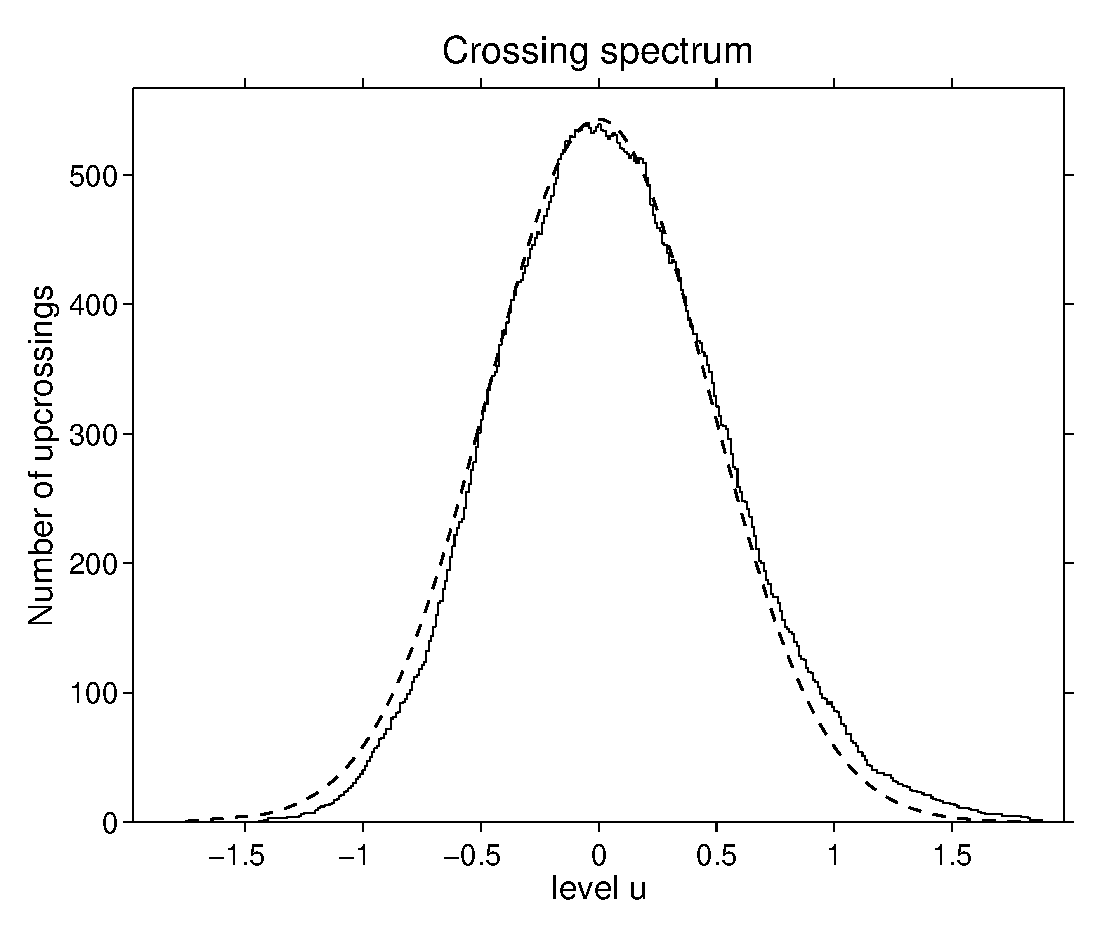
\includegraphics[width=\narrowfigwidth]{fig1_cr}
\vspace{-3mm}
\caption[Example of crossing spectrum]{
The observed crossings intensity compared with the theoretically expected for
Gaussian signals, see (\ref{eq:rice}).}
\label{fig1_cr}
\end{figure}
The process of fatigue damage accumulation depends only on the values
and the order of the local extremes in the load. The sequence of local
extremes is called the \emph{sequence of turning points}.
\index[xentr]{turning points}
\index[xentr]{sequence of turning points} It is a two
column matrix with time for the extremes in the first column and the
values of the extremes in the second.
{\small\begin{verbatim}
      tp = dat2tp(xx);
      fm = length(tp)/(2*T)            % frequency of maxima
      alfa = f0/fm
\end{verbatim}}\index[xcmds]{{\tt dat2tp}}

Here {\tt alfa} is the irregularity factor. Note that {\tt length(tp)} is
equal to the number of local maxima and minima and hence we have a
factor~2 in the expression for {\tt fm}.
\end{rtex}

We finish this section with some remarks about the quality
of the measured data. Especially sea surface measurements can be
of poor quality.
It is always good practice to visually examine the data
before the analysis to get an impression of the quality,
non-linearities and narrow-bandedness of the data.

\begin{cex}{Ex_sea_statistics}\label{page:spurious}
First we shall plot the data {\tt xx} and zoom in on a specific region.
A part of the sea data is presented in Figure~\ref{fig2-1}
obtained by the following commands.
 {\small\begin{verbatim}
      waveplot(xx,tp,'k-','*',1,1)
      axis([0 2 -inf inf])
\end{verbatim}}\index[xcmds]{{\tt waveplot}}

\begin{figure}
\centering
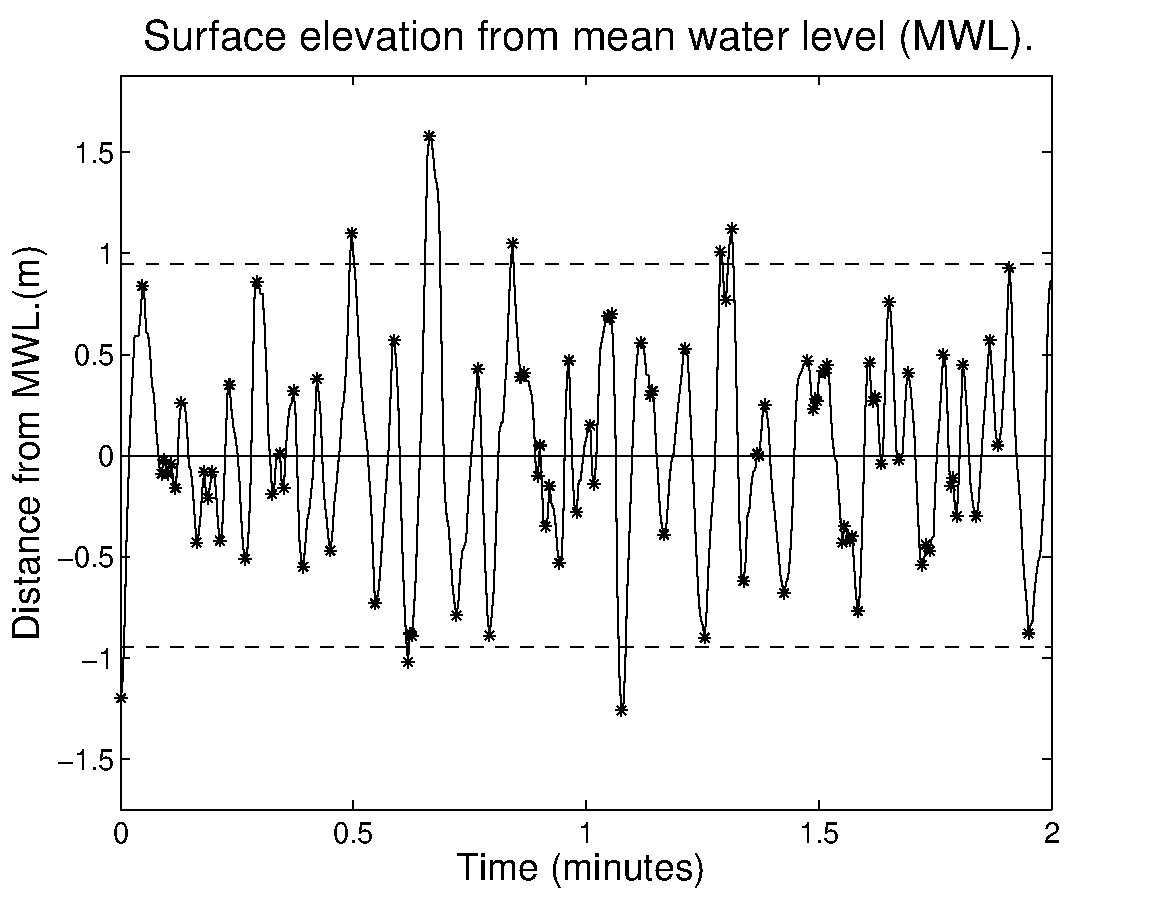
\includegraphics[width=\narrowfigwidth]{figure_Ch2_1}
\vspace{-3mm}
\caption[Plotting sea data and local turning points]{A part of
the sea data with turning points marked as stars.}
\label{fig2-1}
\end{figure}

However, if the amount of data is too large for visual examination, or
if one wants a more objective measure of the quality of
the data, one could use the following empirical criteria:
\begin{itemize}\setlength\itemsep{-1mm}
\item $x'(t) < 5$ [m/s], since the raising speed of
Gaussian waves rarely exceeds 5 [m/s],
\item $x''(t) < 9.81/2$, $[m/s^2]$ which is the limiting maximum
acceleration of Stokes waves,
\item if the signal is constant in some intervals, then this will add high
frequencies to the estimated spectral density; constant data may occur if
the measuring device is blocked during some period of time.
\end{itemize}

\noindent
To find possible spurious points of the dataset use the following commands.
{\small\begin{verbatim}
      dt = diff(xx(1:2,1));
      dcrit = 5*dt;
      ddcrit = 9.81/2*dt*dt;
      zcrit = 0;
      [inds indg] = findoutliers(xx,zcrit,dcrit,ddcrit);
\end{verbatim}}\index[xcmds]{{\tt findoutliers}}

\noindent
The program will give the following list when used on the sea data.
{\small\begin{verbatim}
Found 0 missing points
Found 0 spurious positive jumps of Dx
Found 0 spurious negative jumps of Dx
Found 37 spurious positive jumps of D^2x
Found 200 spurious negative jumps of D^2x
Found 244 consecutive equal values
Found the total of 1152 spurious points
\end{verbatim}}

The values for {\tt zcrit}, {\tt dcrit} and  {\tt ddcrit}
can be chosen more carefully. One must be careful using the
criteria for extreme value analysis, because
it might remove extreme waves that belong to the data and
are not spurious. However, small changes of the
constants are usually not so crucial. As seen from the
transcripts from the program a total of 1152 points are
found to be spurious which is approximately 12~\% of the data.
Based on this one may classify the datasets into good,
reasonable, poor, and useless. Obviously, uncritical use of
data may lead to unsatisfactory results. We return to this
problem when discussing methods to reconstruct the data.
\end{cex}

\section{Frequency modelling of load histories}
\label{sec:freq-model-load}

\subsection{Power spectrum, periodogram}\label{powerspectrum}
The most important characteristic of signals
of the form (\ref{eqn:fourier_series})
in frequency domain is their power
spectrum  \index[xentr]{power spectrum}\index[xentr]{spectrum!power}
$$\hat{s}_i=(a_i^2+b_i^2)/(2\Delta\omega),$$
where $\Delta\omega$ is the sampling interval in frequency
domain, i.e.\ $\omega_i=i\cdot \Delta\omega$.
The two-column matrix $\hat{s}(\omega_i)=(\omega_i,\hat{s}_i)$
will be called the {\it power spectrum} of $x(t)$. The alternative term
{\it periodogram} was introduced as early as 1898 by A.\ Schuster,
\cite{Schuster}. \index[xentr]{periodogram}

The sequence $\theta_i$ such that
$\cos \theta_i = a_i/\sqrt{2\, \hat{s}_i\, \Delta\omega}$ and
$\sin \theta_i = - b_i/\sqrt{2\, \hat{s}_i\, \Delta\omega}$,
is called a sequence of
phases and the Fourier series can be written as follows:
$$
x(t)\approx m + \sum_{i=1}^N \sqrt{2\, \hat{s}_i\Delta\omega}
\cos(\omega_i\,t+\theta_i).
$$
If the sampled signal contains
exactly $2N+1$ points, then $x(t)$ is equal to its Fourier series at the
sampled points. In the special case when $N=2^k$, the so-called FFT
(Fast Fourier Transform) can be used to compute the Fourier
coefficients (and the spectrum) from the measured signal and in
reverse the signal from the Fourier coefficients.

The Fourier coefficient to the zero frequency
is just the mean of the signal, while the variance is given by
$\sigma^2=\Delta\omega\sum \hat{s}(\omega_i)
\approx \int_0^\infty \hat{s}(\omega)\, \rd\omega$. The last integral
is called the zero-order spectral moment $m_0$. Similarly,
higher-order spectral moments are defined by \index[xentr]{spectrum!moments}
$$
m_n=\int_0^\infty \omega^n \, \hat{s}(\omega)\, \rd \omega.
$$

\begin{figure}[t]
\centering
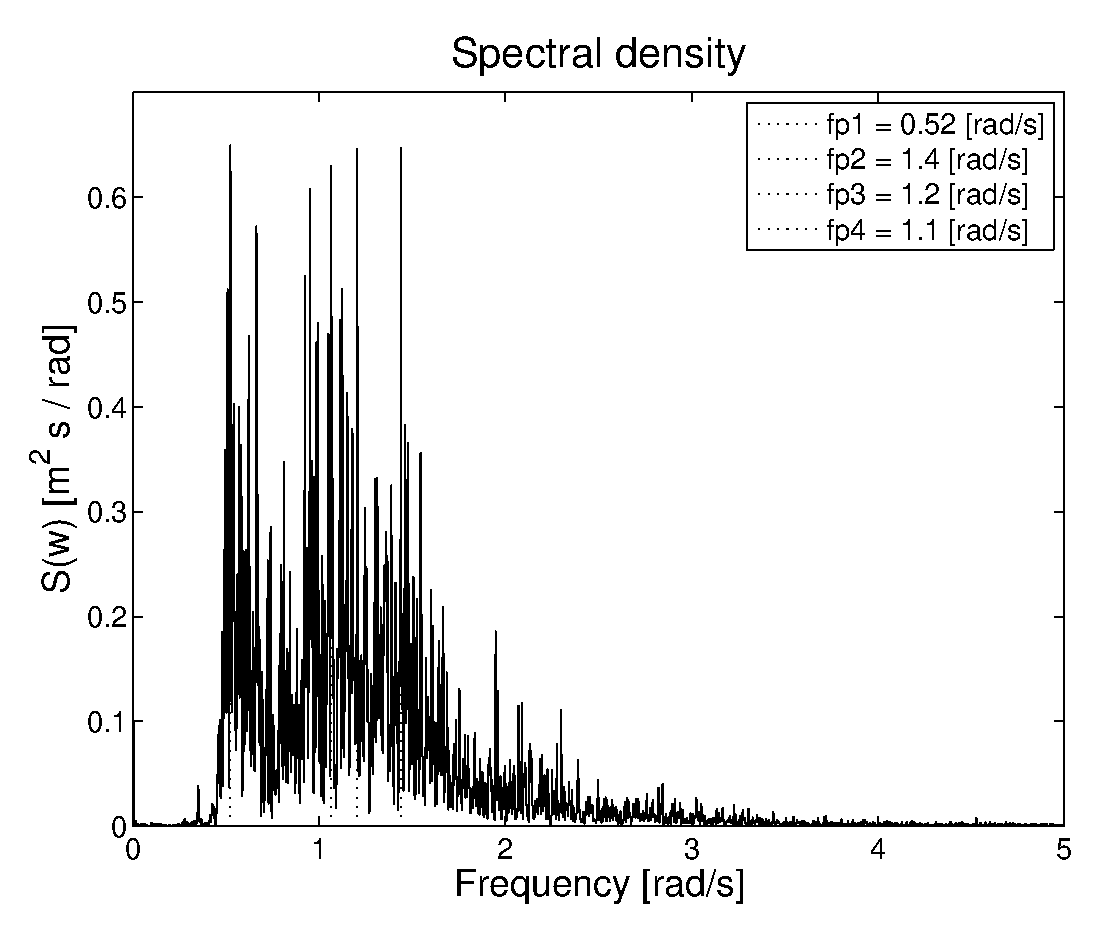
\includegraphics[width=\narrowfigwidth]{fig1_spc}
\vspace{-3mm}
\caption[Non-smoothed spectrum of  {\tt sea.dat}]{
The observed, unsmoothed,  spectrum in the data set {\tt sea.dat}.}
  \label{fig1_spc}
\end{figure}

\begin{cex}{Ex_sea_statistics}
We now calculate the spectrum $\widehat{s}(\omega)$ for the
sea data signal {\tt xx}. \index[xcmds]{{\tt dat2spec}}
{\small\begin{verbatim}
      Lmax = 9500;
      SS = dat2spec(xx,Lmax);
      plotspec(SS); axis([0 5 0 0.7])
\end{verbatim}}\index[xcmds]{{\tt dat2spec2}}

The produced plot, not reproduced in this tutorial, shows the spectrum 
$\widehat{s}(\omega)$ in blue surrounded by 95\% confidence limits, 
in red. These limits can be removed by the command
{\small\begin{verbatim}
      SS = rmfield(SS,'CI')
      plotspec(SS); axis([0 5 0 0.7])
\end{verbatim}}
\noindent giving Figure~\ref{fig1_spc} where we can see that the 
spectrum is extremely
irregular with sharp peaks at many distinct frequencies.
In fact, if we had analysed another section of the sea data we had
found a similar general pattern, but the sharp peaks had been found at
some other frequencies. It must be understood, that the observed
irregularities are random and vary between measurements of the sea
even under almost identical conditions.
This will be further discussed in the following section, where we
introduce smoothing techniques to get a stable spectrum that
represents the ``average randomness'' of the sea state.

Next, the spectral moments will be computed.
{\small\begin{verbatim}
      [mom text] = spec2mom(SS,4)
      [sa sqrt(mom(1))]
\end{verbatim}}\index[xcmds]{{\tt spec2mom}}
The vector {\tt mom} now contains spectral moments $m_0, m_2, m_4$,
which are the variances of the signal and its  first and second
derivative. We can speculate that the variance of
the derivatives is too high because of spurious points.
For example, if there are several points with the same
value, the Gibb's phenomenon leads to high frequencies in the spectrum.
\end{cex}

\subsection{Gaussian processes in spectral domain}
In the previous section we studied the properties of one specific signal
in frequency domain. Assume now that we get a new series of measurements
of a signal, which we are willing to consider as equivalent to the
first one. However, the two series are seldom identical and differ in
some respect that it is natural to regard as purely random.
Obviously it will have a different spectrum $\hat{s}(\omega)$
and the phases will be changed.

A useful mathematical model for such a situation is the random
function (stochastic process) model which will be denoted by $X(t)$.
Then $x(t)$ is seen as particular randomly chosen function.
The simplest model for a stationary signal with a fixed
spectrum $\hat{s}(\omega)$ is
\begin{equation}
X(t)= m + \sum_{i=1}^N \sqrt{\hat{s}_i\, \Delta\omega} \,
\sqrt{2}\cos(\omega_i\,t+\Theta_i),
\label{eqn:sum_with_random_phases}
\end{equation}
where the phases $\Theta_i$ are random variables, independent and
uniformly distributed between $0$ and $2 \pi$.
However, this is not a very realistic model either, since in
practice one often observes a variability in the spectrum amplitudes 
$\hat{s}(\omega)$ between measured functions. Hence, $\hat{s}_i$
should also be modelled to include a certain randomness.

The best way to accomplish this realistic variability  
is to assume that there exists
a deterministic function $S(\omega)$ such that the {\it average value}
of $\widehat{s}(\omega_i)\Delta\omega$ over many observed series
can be approximated by $S(\omega_i)\Delta\omega$. In fact,
in many cases one can model the variability of $\hat{s}_i$ as
$$\hat{s}_i=R_i^2\cdot S(\omega_i)/2,$$
where $R_i$ are independent random factors, all with a Rayleigh distribution,
with probability density function $f_R(r)=r \exp (-r^2/2), r > 0$.
(Observe that the average value of $R_i^2$ is 2.)
This gives the following random function as a model for the series,
\begin{equation}
X(t)= m +
\sum_{i=1}^N \sqrt{S(\omega_i)\, \Delta\omega}\,
R_i\cos(\omega_i\,t+\Theta_i). \label{discretespectrumprocess}
\end{equation}
The process $X(t)$ has many useful properties that can be used for
analysis. In particular, for any fixed $t$, $X(t)$ is normally (Gaussian)
distributed. Then, the probability of any event defined for $X(t)$
can, in principle, be computed when the mean $m$ and the spectral
density $S$ are known.

In sea modelling, the components in the sum defining $X(t)$ can be
interpreted as individual waves. The assumption that $R_i$ and
$\Theta_i$ are independent random variables implies that
the individual waves are independent stationary
Gaussian processes\footnote{A \emph{Gaussian} stochastic process $X(t)$ is
any process such that all linear combinations $\sum a_k X(t_k)$ have a
Gaussian distribution; also derivatives $X'(t)$ and
integrals $\int_a^b X(t)\, \rd t$
are Gaussian.}
with mean zero and covariance function given by
$$
r_i(\tau) = \Delta\omega \, S(\omega_i) \cos(\omega_i\,\tau).
$$
Consequently, the covariance between $X(t)$ and $X(t+\tau)$
is given by
$$
r_X(\tau) = \ex [(X(t)-m)(X(t+\tau)-m)]=\Delta\omega \,\sum_{i=1}^N  S(\omega_i)
\cos(\omega_i\,\tau).
$$
A process like \eqref{discretespectrumprocess}, which is the sum of discrete terms, 
is said to have discrete spectrum. \index[xentr]{spectrum!discrete} Its total energy 
is concentrated to a set of distinct frequencies. 

More generally, for a stationary stochastic process with spectral density
$S(\omega)$, the covariance function $r(\tau)$\index[xentr]{covariance function}  
of the process is defined
by its spectral density function $S(\omega)$,\index[xentr]{spectral density!function} 
also called power spectrum,
\begin{equation}
r(\tau) = \co [X(t), X(t+\tau)] = \int_0^\infty \cos(\omega\tau)
\,S(\omega) \, \rd \omega. \label{spec2cov}
\end{equation}
Since $\va [X(t)] = r_X(0) = \int_0^\infty S(\omega)\, \rd \omega$,
the spectral density represents a continuous distribution of the wave energy
over a continuum of frequencies. The spectrum is continuous. 
\index[xentr]{spectrum!continuous}
\index[xentr]{covariance function!computation from spectrum}

The covariance function and the spectral density form a 
{\it Fourier transform pair}. The spectral density can 
be \index[xentr]{spectrum!computation from covariance function}
computed from the covariance function by the Fourier inversion formula, 
which for continuous-time signals reads,\index[xentr]{Fourier inversion}
\begin{equation}
S(\omega) = \frac{2}{\pi} \int_0^\infty \cos (\omega  \tau) r(\tau)\, \rd \tau.
\label{cov2spec}
\end{equation}

The Gaussian process model is particularly useful in connection
with linear filters. \index[xentr]{linear filter}
If $Y(t)$ is the output of a linear filter
with the Gaussian process $X(t)$ as input,
then  $Y(t)$ is also normally distributed.
Further, the spectrum of $Y(t)$ is related to that of $X(t)$ in
a simple way. If the filter has {\em transfer function}
$H(\omega)$, also called \index[xentr]{transfer function}
{\em frequency function}, \index[xentr]{frequency function}
then the spectrum of $Y(t)$, denoted by $S_Y$,
is given by
$$S_Y(\omega)=|H(\omega)|^2S_X(\omega).$$

For example, the derivative $X'(t)$ is a Gaussian process
with mean zero and spectrum $S_{X'}(\omega)=\omega^2S_X(\omega)$.
The variance of the derivative is equal to the second spectral moment,
$$
\sigma_{X'} ^2=\int S_{X'}(\omega)\, \rd\omega =
\int \omega ^2 S_X(\omega)\, \rd\omega = m_2.
$$

\begin{figure}[tbh]
\centering
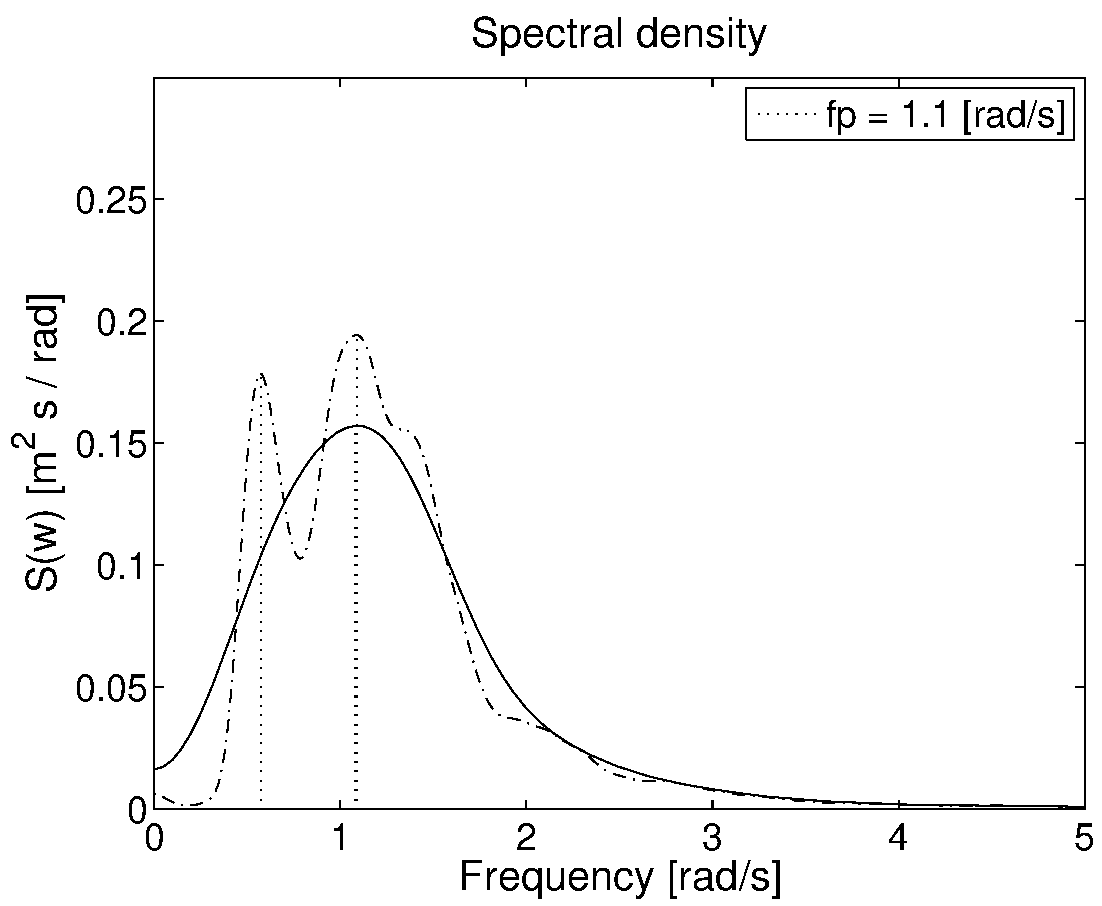
\includegraphics[width=\narrowfigwidth]{fig2_spc}
\vspace{-3mm}
\caption[Spectra  of {\tt sea.dat} with varying degree of smoothing]{
Estimated spectra {\tt SS1, SS2} for the data set {\tt sea.dat}
with varying degree of smoothing; dash-dotted: {\tt Lmax1 = 200}, solid: {\tt Lmax2 = 50}.}
  \label{fig2_spc}
\end{figure}

\begin{cex}{Ex_sea_statistics}
In order to estimate the spectrum of a Gaussian process one needs\index[xentr]{spectrum!estimation of}
  \index[xentr]{spectral density!estimation}
several realizations of the process. Then, one spectrum estimate can be
made for each realization, which are then averaged. However, in many cases
only one realization of the process is available. In such a case
one is often assuming that the spectrum is a smooth function of $\omega$
and one can use this information to improve the estimate. In practice,
it means that one has to use some smoothing techniques.
For the {\tt sea.dat} we shall estimate the spectrum
by means of the \progname{} function
{\tt dat2spec}\index[xcmds]{{\tt dat2spec}}
with a second parameter defining the degree of smoothing.\label{page:SS1}
{\small\begin{verbatim}
      Lmax1 = 200; 
      Lmax2 = 50;
      SS1 = dat2spec(xx,Lmax1);
      SS2 = dat2spec(xx,Lmax2);
      plotspec(SS1,[],'-.'), hold on
      plotspec(SS2), hold off
\end{verbatim}}
\noindent In Figure~\ref{fig2_spc}
we see that with decreasing second input the spectrum estimate becomes 
smoother, and that in the end it becomes unimodal.

An obvious question after this exercise is the following: Which of the two estimates in 
Figure~\ref{fig2_spc} is more correct, in the sense that it best reflects 
important wave characteristics? Since the correlation structure is a very 
important characteristic, we check which spectrum can best reproduce the 
covariance function of the data {\tt xx}. 

The following
code in \progname{} will compute the covariance for the bimodal spectral
density {\tt S1}\index[xcmds]{{\tt covplot}}\index[xcmds]{{\tt spec2cov}}\index[xcmds]{{\tt dat2cov}}
and compare it with the estimated covariance in the signal {\tt xx}.
{\small\begin{verbatim}
      Lmax = 80;
      R1 = spec2cov(SS1,1);
      Rest = dat2cov(xx,Lmax);
      covplot(R1,Lmax,[],'.'), hold on
      covplot(Rest), hold off
\end{verbatim}}
\noindent With the unimodal spectrum {\tt SS2} instead of {\tt SS1} we also compute the 
covariance function {\tt R2 = spec2cov(SS2,1)} and plot it together with {\tt Rest}.  

We can see in Figure~\ref{fig4_s2c}(a)
that the covariance function corresponding to the spectral density {\tt SS2}
differs significantly from the one estimated directly from data.
The covariance corresponding to {\tt SS1} agrees much
better with the estimated covariance function, as seen in Figure~\ref{fig4_s2c}(b). 
Our conclusion is that the bimodal spectrum in Figure~\ref{fig2_spc} is a better 
model for the data {\tt sea.dat} than the unimodal one. 
~ \end{cex}

\begin{figure}
\subfigure[]{%
\label{fig4_s2ca}
\begin{minipage}[b]{0.49\textwidth}%
\centering 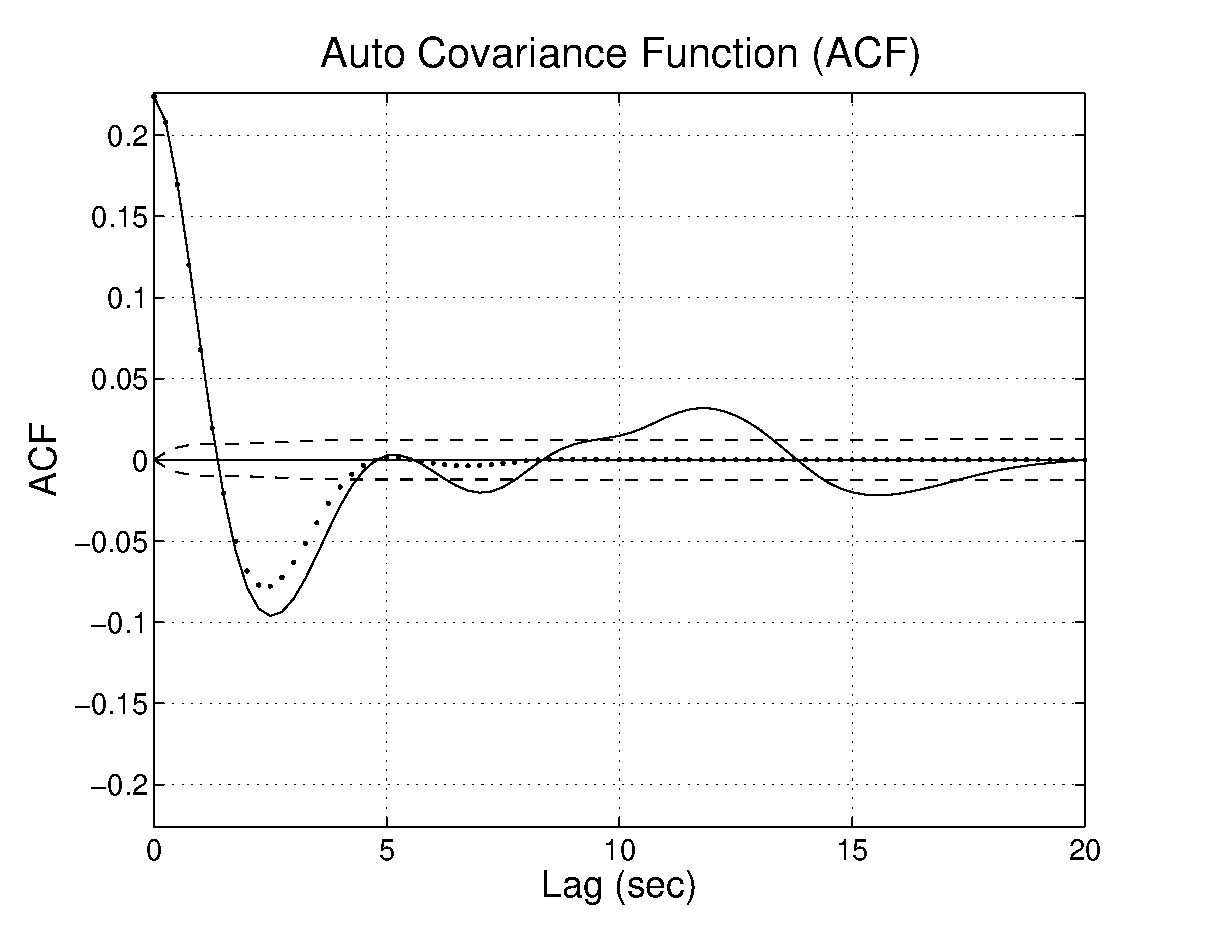
\includegraphics[width=\defwidth]{fig4_s2cb}
\end{minipage}}%
\hfill
\subfigure[]{%
\label{fig4_s2cb}
\begin{minipage}[b]{0.49\textwidth}%
\centering 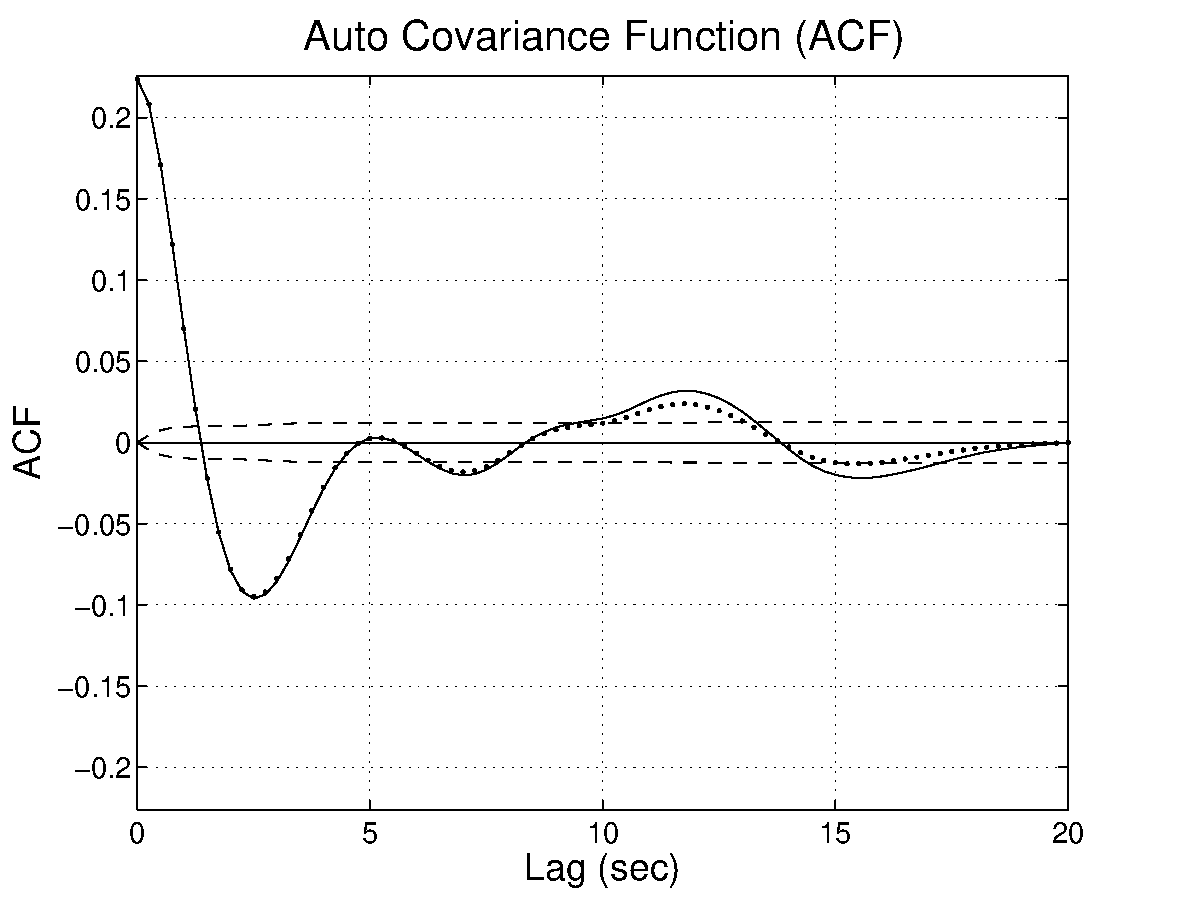
\includegraphics[width=\defwidth]{fig4_s2ca}
\end{minipage}}
\vspace{-3mm}
\caption[ACF computed from spectra of
{\tt sea.dat} with smoothing]{
The covariance function estimated in the data set {\tt sea.dat}, solid line,
compared to the theoretically computed covariance functions for the spectral
densities {\tt SS2} in (a) and {\tt SS1} in (b).
}
  \label{fig4_s2c}
\end{figure}

Observe that the \progname{} function {\tt spec2cov} can be used to compute
a covariance structure which can contain covariances both in time and in
space as well as that of the derivatives.
The input can be any spectrum structure, e.g.\ wavenumber spectrum,
directional spectrum or encountered directional spectrum;
type {\tt help spec2cov} for detailed information.

\subsection{Crossing intensity -- Rice's formula}
\label{subsec:crossing_intensity}
\index[xentr]{Rice's formula}
The Gaussian process is a sum (or in fact an integral) of cosine terms with amplitudes defined
by the spectrum, and the instantaneous value $X(t)$ has a normal distribution
with mean $0$ and variance $\sigma^2 = \int S(\omega)\, \rd \omega$. 
The spectral density $S(\omega)$ determines the relative importance of 
components with different frequencies. 

In wave analysis and fatigue applications there is another quantity that
plays a central role, namely the {\em upcrossing intensity} $\mu(u)$,
which yields the average number, per time or space unit,
of upcrossings of the level $u$. It
contains important information on the fatigue properties of a
load signal and also of the wave character of a random wave.\footnote{%
The general expression for the upcrossing intensity for a stationary process
 is
$\mu(u)=\int_{z=0}^\infty z\, f_{X(0),X'(0)}(u,z)\, \rd z$, where
$f_{X(0),X'(0)}(u,z)$ is a joint probability density function.}

For a Gaussian process the crossing intensity
is given by the celebrated {\it Rice's formula},
\index[xentr]{Rice's formula}
\begin{equation}
\mu(u)=f_0\exp\left\{-\frac{(u-m)^2}{2\sigma^2}\right\}.\label{eq:rice}
\end{equation}
Using spectral moments we have that $\sigma^2=m_0$ while
$f_0=\frac{1}{2\pi}\sqrt{\frac{m_2}{m_0}}$ is the mean frequency.
\index[xentr]{mean frequency}

\subsection{Transformed Gaussian models}\label{ss:transformedGaussianmodels}
\index[xentr]{transformed Gaussian models|(}

The standard assumptions for a sea state under stationary conditions are
that $X(t)$ is a stationary and ergodic stochastic process with
mean $\ex[X(t)]$ assumed to be zero, and with a spectral density
$S(\omega)$. The knowledge of which kind of spectral densities
$S(\omega)$ are suitable to describe different sea state data is well
established from experimental studies.

Real data $x(t)$ seldom perfectly support the Gaussian assumption for
the process $X(t)$. But since the Gaussian case is well understood
and there are approximative methods to obtain wave characteristics
from the spectral density $S(\omega)$ for Gaussian processes,
one often looks for a model of the sea state in the
class of Gaussian processes. Furthermore, in previous work,
\cite{RychlikEtal1997Modelling},
%,RyLJ97} %Rychlik, Leadbetter and Johannesson 1997
we have found that for many sea wave data, even such that are clearly
non-Gaussian, the wavelength and amplitude densities can be very
accurately  approximated using the Gaussian process model.

However, the Gaussian model can lead to less satisfactory results
when it comes to the distribution of crest heights or joint densities
of troughs and crests. In that case we found in
\cite{RychlikEtal1997Modelling}
that a simple transformed Gaussian process used to model $x(t)$ gave
good approximations for those densities.

Consequently, in \progname{} we shall model $x(t)$ by a process $X(t)$ which is a
function of a single Gaussian process $\widetilde X (t)$, i.e.\
\begin{equation}\label{eq:trprocess}
X(t)=G(\widetilde X(t)),
\end{equation}
where $G(\cdot)$ is a continuously differentiable function with
positive derivative.  We shall denote the spectrum of $X$ by $S$,
and the spectrum of $\widetilde X (t)$ by $\widetilde S$.
The transformation $G$ performs the appropriate non-linear
translation and scaling so that $\widetilde X(t)$ is always normalized to
have mean zero and variance one, i.e.\ the first spectral moment of
$\widetilde S$ is one.

Note that once the distributions of crests, troughs, amplitudes or
wavelengths in a Gaussian process $\widetilde X (t)$ are computed, then
the corresponding wave distributions in $X(t)$ are obtained by a simple
variable transformation involving only the inverse of $G$, which we
shall denote by $g$. Actually we shall use the function $g$ to define
the transformation instead of $G$, and use the relation $\widetilde x
(t) = g(x(t))$ between the real sea data $x(t)$ and the transformed
data $\widetilde x (t)$.
If the model in Eq.~(\ref{eq:trprocess}) is correct, then
$\widetilde x(t)$ should be a sample function of a process with
Gaussian marginal distributions.
%Obviously, a Gaussian model is
%obtained by using a linear function $g(y)=ay + b$, where $a, b$ are
%constants.

There are several different ways to proceed when selecting a transformation.
The simplest alternative is to estimate the function
$g$ directly from data by some parametric or non-parametric techniques. A more
physically motivated procedure is to use some of the parametric functions
proposed in the literature, based on approximations of non-linear wave
theory.  The following options are programmed in the
toolbox:
{\small\begin{verbatim}
      dat2tr    - non-parametric transformation g proposed by Rychlik,
      hermitetr - transformation g proposed by Winterstein,
      ochitr    - transformation g proposed by Ochi et al.
\end{verbatim}}
\index[xentr]{transformed Gaussian models!Winterstein}
\index[xentr]{transformed Gaussian models!Ochi et al.}
\index[xentr]{transformed Gaussian models!Rychlik}
\index[xentr]{transformed Gaussian models!nonparametric}
\index[xcmds]{{\tt hermitetr}}
\index[xcmds]{{\tt ochitr}}
\index[xcmds]{{\tt dat2tr}}

The transformation proposed by by Ochi et al.,
\cite{OchiAndAhn1994Probability},
is a monotonic exponential function, while Winterstein's model,
\cite{Winterstein1988Nonlinear}, is a
monotonic cubic Hermite polynomial. Both transformations use higher moments
of $X(t)$ to compute $g$. Information about the moments of the process
can be obtained by site specific data, laboratory measurements or from
physical considerations. Rychlik's non-parametric method is based on
the crossing intensity $\mu(u)$; see \cite{RychlikEtal1997Modelling}.
Martinsen and Winterstein, \cite{MarthinsenAndWinterstein1992Skewness},
derived an expression for the
skewness and kurtosis for narrow banded Stokes waves to the leading order
and used these to define the transformation.
The skewness and kurtosis (excess) of this model can also be estimated from
data by the \progname{} functions {\tt skew}
\index[xcmds]{{\tt skew}}
and {\tt kurt}\index[xcmds]{{\tt kurt}}.

\begin{cex}{Ex_sea_statistics}
We begin with computations of skewness and kurtosis
for the data set {\tt xx}. The commands
{\small\begin{verbatim}
      rho3 = skew(xx(:,2))
      rho4 = kurt(xx(:,2))
\end{verbatim}}
\noindent
give the values {\tt rho3 = 0.25} and {\tt  rho4 = 3.17},
respectively, compared to {\tt rho3 = 0} and  {\tt rho4 = 3}
for Gaussian waves. We can compute the same model for
the spectrum $\tilde S$ using the second order wave approximation
proposed by Winterstein. His approximation gives suitable
values for skewness and kurtosis
{\small\begin{verbatim}
      [sk, ku] = spec2skew(S1);
\end{verbatim}}\index[xcmds]{{\tt spec2skew}}

Here we shall use Winterstein's Hermite transformation
and denote it by {\tt gh},
and compare it with the linear transformation, denoted by {\tt g}, that
only has the effect to standardize the signal, assuming it is already Gaussian,
{\small\begin{verbatim}
      gh = hermitetr([],[sa sk ku me]);
      g  = gh; g(:,2)=g(:,1)/sa;
      trplot(g)
\end{verbatim}}\index[xcmds]{{\tt hermitetr}}
\noindent These commands will result in two two-column matrices,
{\tt g, gh}, with equally spaced $y$-values in the first column
and the values of $g(y)$ in the second column.

Since we have data we may estimate the transformation directly by the method
proposed by Rychlik et al., in \cite{RychlikEtal1997Modelling}:
{\small\begin{verbatim}
      [glc test0 cmax irr gemp] = dat2tr(xx,[],'plotflag',1);
      hold on
      plot(glc(:,1),glc(:,2),'b-')
      plot(gh(:,1),gh(:,2),'b-.'), hold off
\end{verbatim}}\index[xcmds]{{\tt dat2tr}}
\noindent The same transformation can be obtained from data 
and the crossing intensity by use of the \progname{} functions  
{\tt dat2lc} followed by 
{\tt lc2tr}\index[xcmds]{{\tt lc2tr}}\index[xcmds]{{\tt dat2lc}}.

\begin{figure}[thb]
\centering
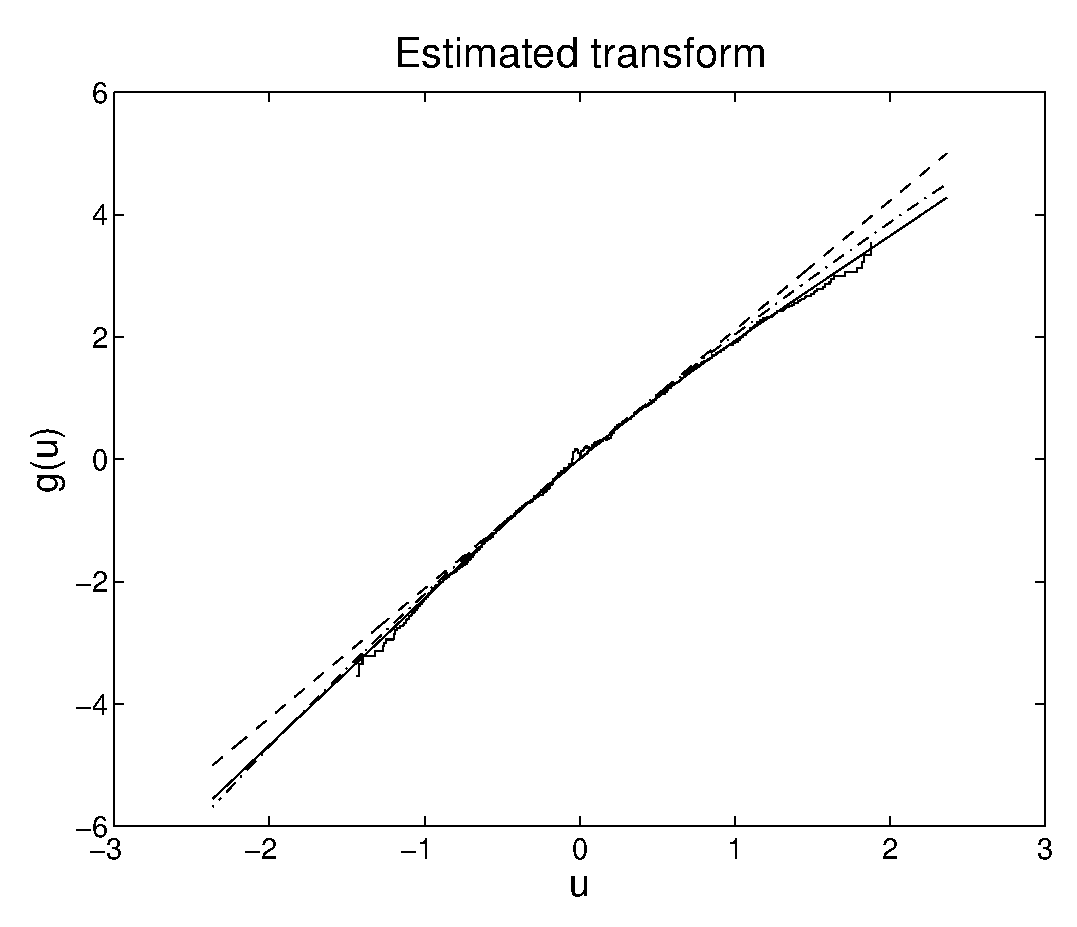
\includegraphics[width=\narrowfigwidth]{fig4_tr}
\vspace{-3mm}
\caption[Comparison of data transformations]{%
Comparisons of the three transformations $g$,
straight line is the Gaussian model,
dash dotted line the Hermite transformation {\tt gh} and solid line the
Rychlik method {\tt glc}.}
  \label{fig4_tr}
\end{figure}

In Figure~\ref{fig4_tr} we compare the three transformations,
the straight line is the Gaussian linear model, the dash dotted
line is the Hermite transformation based on higher moments of the
response computed from the spectrum and the solid line is the direct
transformation estimated from crossing intensity.
(The unsmoothed line shows the estimation of
the direct transformation from unsmoothed crossing intensity).
We can see that the transformation derived from crossings will give
the highest crest heights. It can be proved that asymptotically
the transformation based on crossings intensity gives the
correct density of crest heights.

The transformations indicate that data {\tt xx} has a light
lower tail and heavy
upper tail compared to a Gaussian model.
This is also consistent with  second order wave theory, where the crests
are higher and the troughs shallower compared to Gaussian waves.
Now the question is whether this difference is significant
compared to the natural statistical variability due to finite length
of the time series.

\begin{figure}[t]
\centering
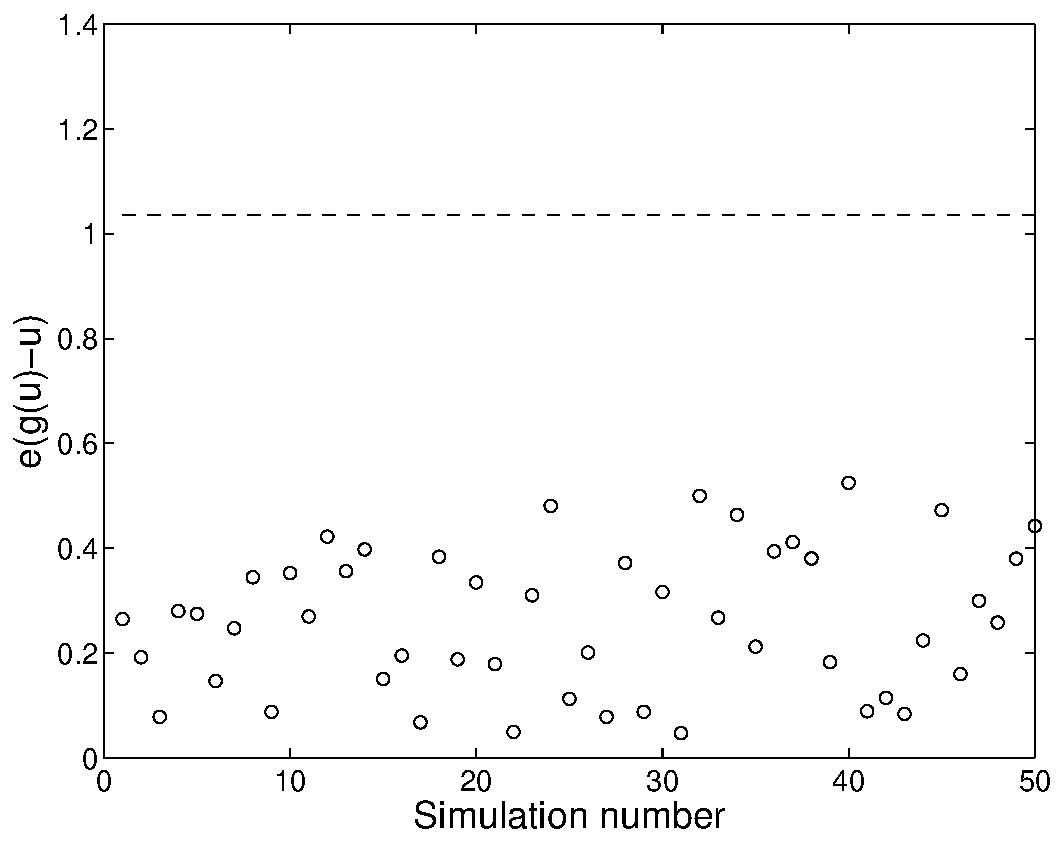
\includegraphics[width=\narrowfigwidth]{figure_Ch2_8}
\vspace{-3mm}
\caption[Simulation technique to test if a stochastic process is Gaussian]{
The simulated 50 values of the {\tt test} variable for
the Gaussian process with spectrum {\tt S1} compared with the
observed value (dashed line).}
  \label{fig2-3}
\end{figure}

To determine the degree of departure from Gaussianity,
we can compare an indicator of non-Gaussianity {\tt test0}
obtained from Monte Carlo simulation. The value
of {\tt test0} is a measure of how munch the transformation {\tt g}
deviates from a straight line.

The significance test is done by simulating 50 independent samples
of {\tt test0} from a true Gaussian process with the same spectral
density and length as the original data. This is accomplished
by the \progname{} program \verb+testgaussian+\index[xcmds]{{\tt testgaussian}}.
The output from the program is
a plot of the ratio \verb+test1+ between the simulated (Gaussian)
{\tt test0}-values and the sample {\tt test0}, that was calculated in the previous call to 
{\tt dat2tr}:
{\small\begin{verbatim}
      N = length(xx);
      test1 = testgaussian(S1,[N,50],test0);
\end{verbatim}}
\noindent
The program gives a plot of simulated {\tt test} values, see
Figure~\ref{fig2-3}. As we see from the figure none of the
simulated values of \verb+test1+ is above 1.00. Thus the data
significantly departs from a Gaussian distribution;
see \cite{RychlikEtal1997Modelling} for more detailed discussion
of the testing procedure and the estimation of the transformation
{\tt g} from the crossing intensity.

We finish the tests for Gaussianity of the data by a more classical
approach and simply plot the data on normal probability paper.
Then $N$ independent observations of identically distributed Gaussian
variables form a straight line in a normalplot.
Now, for a time series the data is clearly not
independent. However, if the process is ergodic then
the data forms a straight line as $N$ tends to infinity.

The command \index[xcmds]{{\tt plotnorm}}
{\small\begin{verbatim}
      plotnorm(xx(:,2))
\end{verbatim}}
\noindent produces Figure~\ref{fig2-4}.
As we can see the normal probability plot is slightly curved
indicating that the underlying distribution has a heavy
upper tail and a light lower tail.
\end{cex}
\begin{figure}[t]
\centering
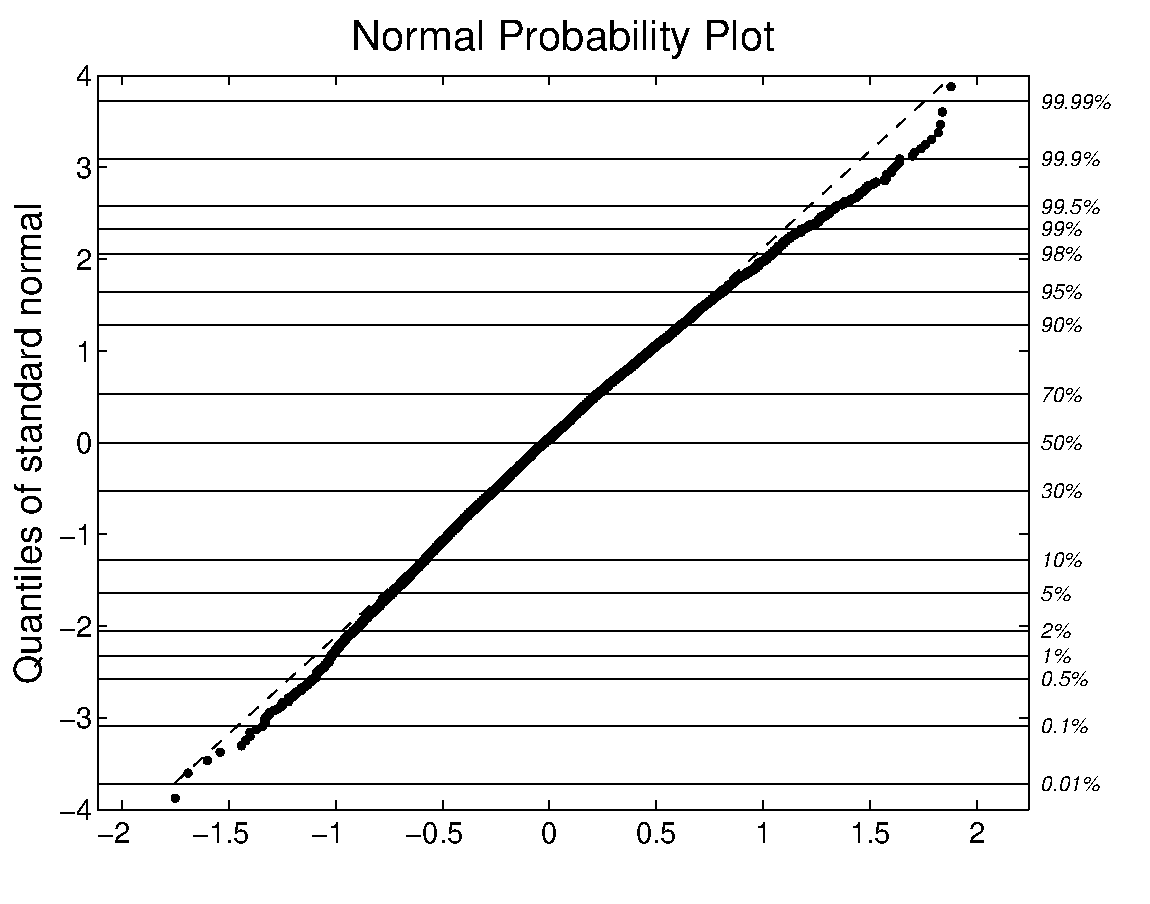
\includegraphics[width=\narrowfigwidth]{figure_Ch2_2}
\vspace{-3mm}
  \caption[Normal probability plot]{The data {\tt sea.dat} on
   normal probability plot.}
  \label{fig2-4}
\end{figure}

\index[xentr]{transformed Gaussian models|)}
\subsection{Spectral densities of sea data}
\index[xentr]{spectrum!of sea data|(}

The knowledge of which kind of spectral density $S(\omega)$ is suitable
to describe sea state data is well established from experimental
studies. One often uses some parametric form of spectral density
functions, e.g.\ a {\sc Jonswap}-spectrum. \index[xentr]{Jonswap spectrum}
This formula is programmed in a \progname{}
function \index[xentr]{spectrum!Jonswap}
{\tt jonswap}, which evaluates the spectral density $S(\omega)$
with specified wave characteristics. There are several other
programmed spectral densities in \progname{} to allow for bimodal and
finite water depth spectra. The list includes the following spectra:
{\small\begin{verbatim}
      jonswap       - JONSWAP spectral density
      wallop        - Wallop spectral density
      ochihubble    - Bimodal Ochi-Hubble spectral density
      torsethaugen  - Bimodal (swell + wind) spectral density
      bretschneider - Bretschneider (Pierson-Moskowitz)
                      spectral density
      mccormick     - McCormick spectral density
      tmaspec       - JONSWAP spectral density
                      for finite water depth
\end{verbatim}}
\index[xcmds]{{\tt jonswap}}\index[xcmds]{{\tt wallop}}
\index[xcmds]{{\tt ochihubble}}\index[xcmds]{{\tt torsethaugen}}
\index[xcmds]{{\tt bretschneider}}\index[xcmds]{{\tt mccormick}}
\index[xcmds]{{\tt tmaspec}}\index[xcmds]{{\tt spec}}
\index[xcmds]{{\tt spreading}}
\progname{} also contains some different spreading functions;
use the help function on {\tt spec} and {\tt spreading}
for more detailed information.

The spectrum of the sea can be given in many different formats,
that are interconnected by the dispersion
relation\footnote{The dispersion relation between frequency
$\omega$ and wavenumber $\kappa$ on finite water depth $h$, reads
$\omega^2=g \kappa \tanh h\kappa$, where $g$ is the acceleration of gravity.}.
The spectrum can be given using
frequencies, angular frequencies or wavenumbers, and it
can also be directional.

A related spectrum is the encountered spectrum for a moving vessel. The
transformations between the different types of spectra
are defined by means of integrals and variable change defined by the
dispersion relation
and the Doppler shift of individual waves.
The function {\tt spec2spec}\index[xcmds]{{\tt spec2spec}}
makes all these transformations easily
accessible for the user. (Actually many programs perform
the appropriate transformations internally whenever it is necessary
and for example one can compute the density of wave-length,
which is a quantity in space domain, from an
input that is the directional frequency spectrum, which is related to the
time domain.)

\begin{figure}[tbh]
\centering
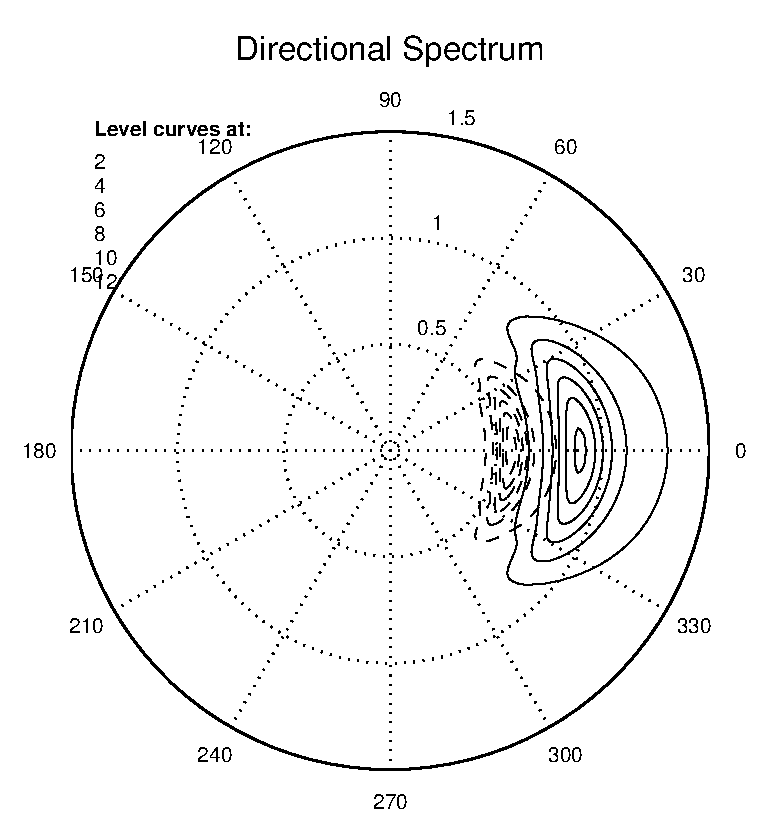
\includegraphics[width=\narrowfigwidth]{figure_spec_enc}
\vspace{-3mm}
\caption[Example of directional spectra]{
Directional spectrum {\tt SJd} of {\sc Jonswap} sea (dashed line)
 compared with the encountered directional spectrum {\tt SJe} for heading sea,
 speed 10 [m/s] (solid line).}
  \label{fig4-5}
\end{figure}

\begin{rtex}{Ex_sea_spectra}{Different forms of spectra}
In this example we have chosen a {\sc Jonswap} spectrum with parameters
defined by significant wave height {\tt Hm0 = 7[m]} and peak period
{\tt Tp = 11[s]}. This spectrum describes the measurements of sea
level at a fixed point (buoy).
{\small\begin{verbatim}
      Hm0 = 7; Tp = 11;
      SJ = jonswap([],[Hm0 Tp]);
      SJ.note
\end{verbatim}} \index[xcmds]{{\tt jonswap}}\index[xentr]{spectrum!Jonswap}

In order to include the space dimension, i.e.\ the direction in which
the waves propagate, we compute a directional spectrum by
adding spreading; see dashed curves in Figure~\ref{fig4-5}.
{\small\begin{verbatim}
      D = spreading(101,'cos2s',0,[],SJ.w,1)
      SJd = mkdspec(SJ,D)  % Directional spectrum
\end{verbatim}}

Next, we consider a vessel moving with
speed {\tt 10[m/s]} against the waves. The sea measured
from the vessel will have a different directional spectrum,
called the encountered  directional spectrum. \index[xentr]{encountered directional spectrum}
The following code will compute the encountered
directional spectrum and plot it on top of
the original spectrum. The result is shown as
the solid curves in Figure~\ref{fig4-5}.
{\small\begin{verbatim}
      SJe = spec2spec(SJd,'encdir',0,10);  % Encountered dir spectrum
      plotspec(SJe), hold on
      plotspec(SJd,1,'--'), hold off
\end{verbatim}} \index[xentr]{spectrum!encountered}
\index[xentr]{spectrum!directional}

Obviously, the periods of waves in the directional sea are defined by
the {\sc Jonswap} spectrum
(in a linear wave model spreading does not affect the sea level at a fixed point),
but the encountered periods will be shorter with heading seas.
This can be seen by comparing the original {\sc Jonswap} spectrum
\verb+SJ+ with the following two point spectra. 
{\small\begin{verbatim}
      SJd1 = spec2spec(SJd,'freq'); % Point spectrum from dir spectrum
      SJd2 = spec2spec(SJe,'enc');  % Point encountered spectrum at ship
      plotspec(SJ), hold on
      plotspec(SJd1,1,'.'),
      plotspec(SJd2), hold off
\end{verbatim}}
\noindent We can see in Figure~\ref{fig4-4}(a) that the spectra
{\tt SJ} and {\tt SJd1} are identical (in numerical sense),
while spectrum {\tt SJd2} contains more energy at higher frequencies.

A similar question is how much the
wave length differs between a longcrested {\sc Jonswap} sea
and a {\sc Jonswap} sea with spreading. The answer lies in 
the {\it wavenumber spectrum}\index[xentr]{spectrum!wavenumber}
that measures how the wave enegy is distributed over different 
wavenumbers, i.e.\ radians (or cycles)  \index[xentr]{wavenumber}
per unit length along a specified direction, usually the main wave direction. 

The wavenumber spectra along the main wave direction 
can be computed by the following  code,
the result of which is shown in Figure~\ref{fig4-4}(b).
{\small\begin{verbatim}
      SJk = spec2spec(SJ,'k1d')  % Unidirectional waves
      SJkd = spec2spec(SJd,'k1d')  % Waves with directional spreading 
      plotspec(SJk), hold on
      plotspec(SJkd,1,'--'), hold off
\end{verbatim}}
\noindent We see how the spreading of energy away from the main direction 
makes observed waves longer. The total energy is of course the same but 
shifted to lower wavenumbers.   

\begin{figure}[tbh]
\subfigure[]{%
\begin{minipage}[b]{0.5\textwidth}%
    \centering   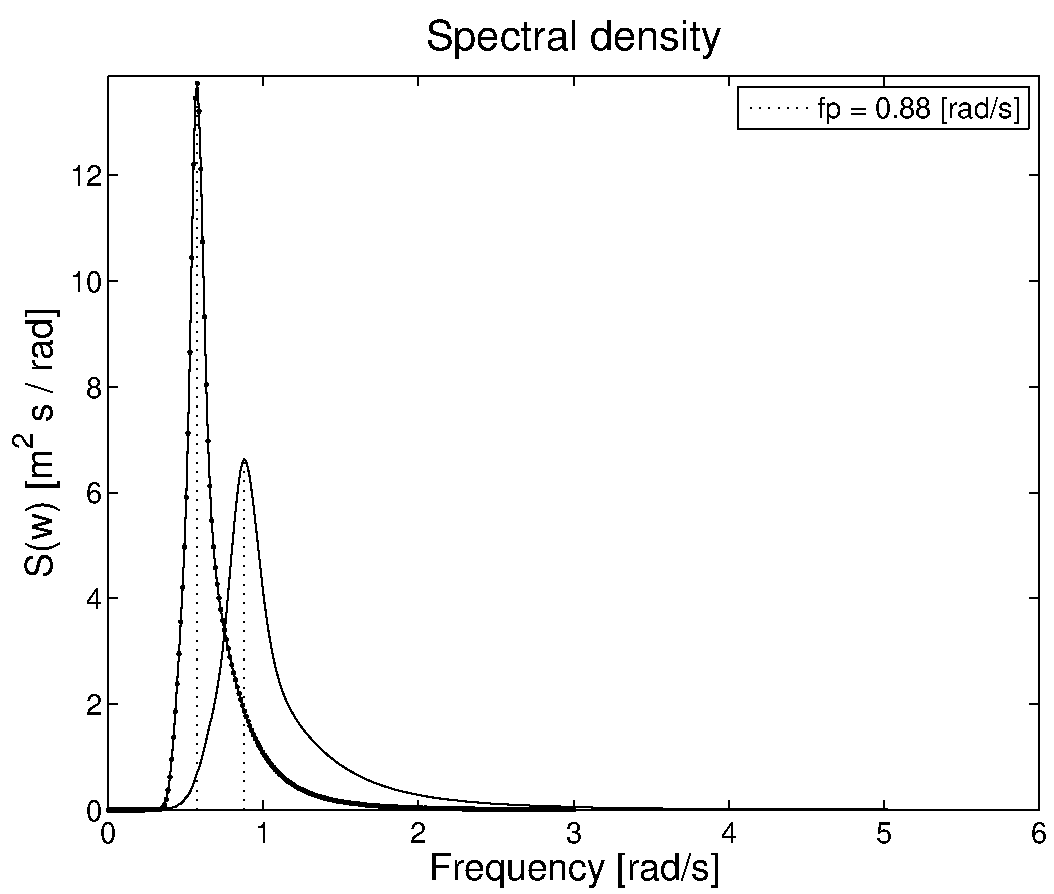
\includegraphics[width=\defwidth]{fig4_Je} %
  \end{minipage}}%
\hfill
\subfigure[]{%
\begin{minipage}[b]{0.5\textwidth}%
    \centering   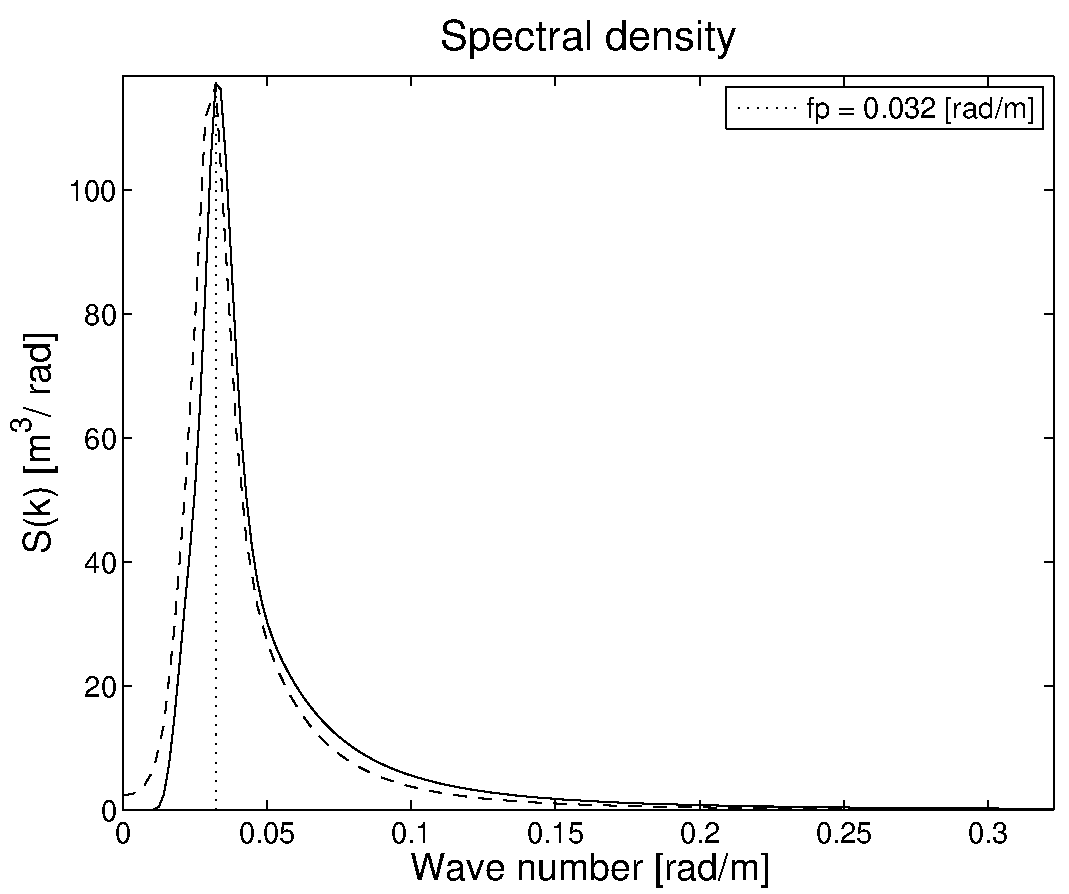
\includegraphics[width=\defwidth]{figure_spec_k1d} %
  \end{minipage}}%
\vspace{-3mm}
\caption[Comparing different forms of spectra]{
 (a) Frequency {\sc Jonswap} spectrum {\tt SJ} and point spectrum 	
 {\tt SJd1} compared with encountered point 
 spectrum {\tt SJd2} for heading sea speed 10 [m/s] (solid line).
(b) Wavenumber spectrum {\tt SJk} for longcrested {\sc Jonswap} sea
(solid line) compared with wavenumber spectrum {\tt SJkd} 
for {\sc Jonswap} with spreading (dashed).
}
  \label{fig4-4}
\end{figure}

Finally, we shall show how the {\sc Jonswap} spectrum
can be corrected  for a finite depth, see \cite{BuowsEtal1985Similarity} for a 
theoretical and empirical study.
The \progname{} function {\tt phi1} computes the frequency dependent 
reduction of the spectrum for waters of finite depth, here 20 meters.
{\small\begin{verbatim}
      plotspec(SJ,1,'--'), hold on
      SJ20 = SJ;
      SJ20.S = SJ20.S.*phi1(SJ20.w,20); % Finite depth correction
      SJ20.h = 20;
      plotspec(SJ20),  hold off
\end{verbatim}} \index[xcmds]{{\tt phi1}}
\noindent The resulting spectra are shown in Figure~\ref{fig4-1}.
\end{rtex}
\begin{figure}[hbt]
\centering
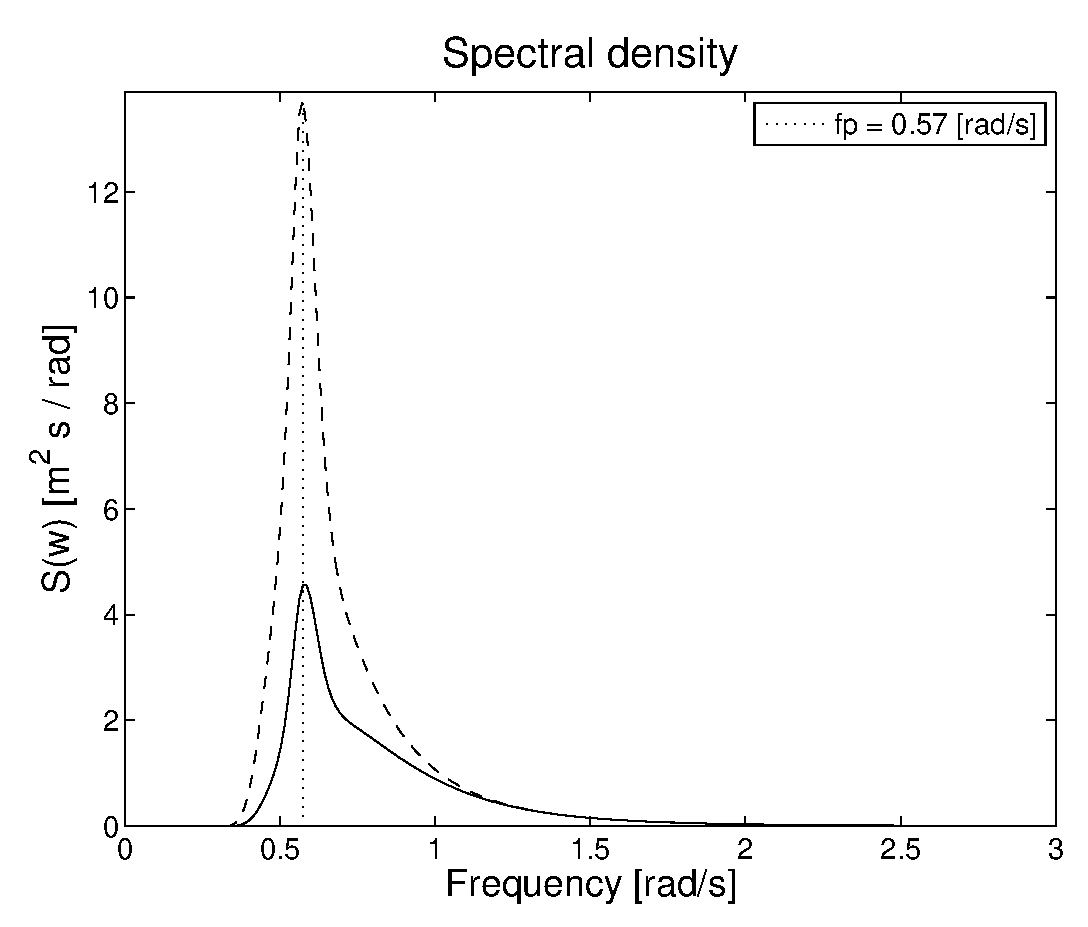
\includegraphics[width=\narrowfigwidth]{figure_spec}
\vspace{-3mm}
  \caption[{\sc Jonswap} spectrum compared
with spectrum on finite depth]{
Standard {\sc Jonswap} spectrum {\tt SJ} (dashed line)
compared with the spectrum {\tt SJ20} on finite depth
of 20 [m] (solid line)
}
  \label{fig4-1}
\end{figure}

\index[xentr]{spectrum!of sea data|)}
\index[xentr]{spectrum!finite depth}

\section{Simulation of transformed Gaussian
  process}\label{sec:simulationofGaussian}
\index[xentr]{transformed Gaussian models|(}
\index[xentr]{transformed Gaussian models!simulation of|(}
\index[xentr]{simulation!of transformed Gaussian process|(}

In this section we shall present some of the programs that can be used to simulate 
%random signals, loads and waves; type {\tt help simtools} for a list.
%We shall be mostly concerned with simulation of the 
the transformed Gaussian model for sea $X(t)=G(\widetilde X(t))$. 
In \progname{} there are several other programs to simulate random functions
or surfaces, both Gaussian and non-Gaussian; use {\tt help simtools}. 
We give examples of some of these functions in Section~\ref{s:2.4}.  

The first important case is when we wish to reproduce random versions
of the measured signal $x(t)$. Using {\tt dat2tr}\index[xcmds]{{\tt dat2tr}}
one first
estimates the transformation {\tt g}. Next, using a function
{\tt dat2gaus}\index[xcmds]{{\tt dat2gaus}}
one can compute $\tilde x(t)=g(x(t))$, which we assume is a realization
of a Gaussian process. From $\tilde x$ we can then estimate
the spectrum $\tilde S(\omega)$ by means of the function
{\tt dat2spec}. The spectrum $\tilde S(\omega)$ and the transformation
$g$ will uniquely define the transformed Gaussian model. A random
function that models the measured signal can then be obtained using the
simulation program {\tt spec2sdat}\index[xcmds]{{\tt spec2sdat}}, 
which includes the desired transformation.
In the following example we shall illustrate
this approach on the data set {\tt sea.dat}.

Before we can start to simulate we need to put the transformation into the
spectrum data structure, which is a \ML{} structure variable; 
see Section~\ref{sec:datastructures}, page~\pageref{sec:datastructures}. 
Since \progname{} is based on transformed Gaussian
processes the entire process structure is defined by the spectrum and
the transformation together. Therefore the transformation has been
incorporated, as part of a model, into the spectrum structure, and is
passed to other \progname{} programs via the spectrum.
If no transformation is given then the process is Gaussian.

Observe that the possibly nonzero mean {\tt m} for the model is
included in the transformation. The change of mean by for example 0.5~[m]
is simply accomplished by modifying the transformation 
by the command {\tt g(:,2) = g(:,2)+0.5;}
Consequently the spectrum structure completely defines the model.

\bigskip
\noindent
{\bf\sc Important note 1:} \label{ImpNote_1} When the simulation routine \verb+spec2sdat+
is called with a spectrum argument that contains a scale changing
transformation \verb+spectrum.tr+, then it is
assumed that the input spectrum is standardized
with spectral moment $m_0=1$, i.e.\ unit variance. The correct
standard deviation
for the output should normally be  obtained via the transformation
\verb+spectrum.tr+. If you happen to use a transformation
{\it together with} an input spectrum that does not have unit
variance, then you get the double scale effect, both from the
transformation and via
the standard deviation from the spectrum. It is only the routine
\verb+spec2sdat+ that works in this way. All other routines, in
particular those which calculate cycle distributions, perform an
internal normalization of the spectrum before the calculation, and
then transforms back to the original scale at the end.

\bigskip
\noindent
{\bf\sc Important note 2:} When you run the simulation examples 
with different time horizon and time step you may experience a
warning

\centerline{
 {\tt 'Spectrum matrix is very large'}.
 }
 
 \noindent
This is a warning from the \wf{} routine {\tt specinterp}, which is used 
internally to adapt the spectrum to the correct Nyquist frequency 
and frequency resolution. You can turn off the warning by commenting 
out three lines in {\tt specinterp} in the {\tt spec} 
module.\index[xcmds]{{\tt specinterp}}

\begin{rtex}{Ex_sea_simulation}{Simulation of a random sea}
\index[xentr]{simulation!of random sea}
In Example~\ref{Ex_sea_statistics} on page~\pageref{page:spurious}
we have shown that the
data set {\tt xx = sea.dat} contains a considerable amount of
spurious points that we would like to omit or censor.

The program \verb+reconstruct+\index[xcmds]{{\tt reconstruct}}
replaces the spurious data by
synthetic data. The new data points are obtained by simulation of 
a conditional Gaussian vector, based on the remaining data, taking the 
fitted transformed Gaussian process model into account; 
see
\cite{BrodtkorbEtal1999Joint,BrodtkorbEtal2001Joint} for more details.
%Brodtkorb et al (1999) for more details)
The reconstruction is performed as
{\small\begin{verbatim}
      [y grec] = reconstruct(xx,inds);
\end{verbatim}}
\noindent
where {\tt y} is the reconstructed data and {\tt grec} is the transformation
estimated from the signal {\tt y}. In Figure~\ref{fig4-11} we can see the
transformation (solid line) compared with the empirical
smoothed transformation,
{\tt glc}, which is obtained from the
original sequence {\tt xx} without removing the spurious data
(dash-dotted line).  We can see that the new transformation
has slightly smaller
crests. Actually, it is almost identical with the transformation
{\tt gh} computed from the spectrum of the signal, however, it
may be only a coincident (due to random fluctuations)
and hence we do not draw any conclusions from this fact.

\begin{figure}
\centering
    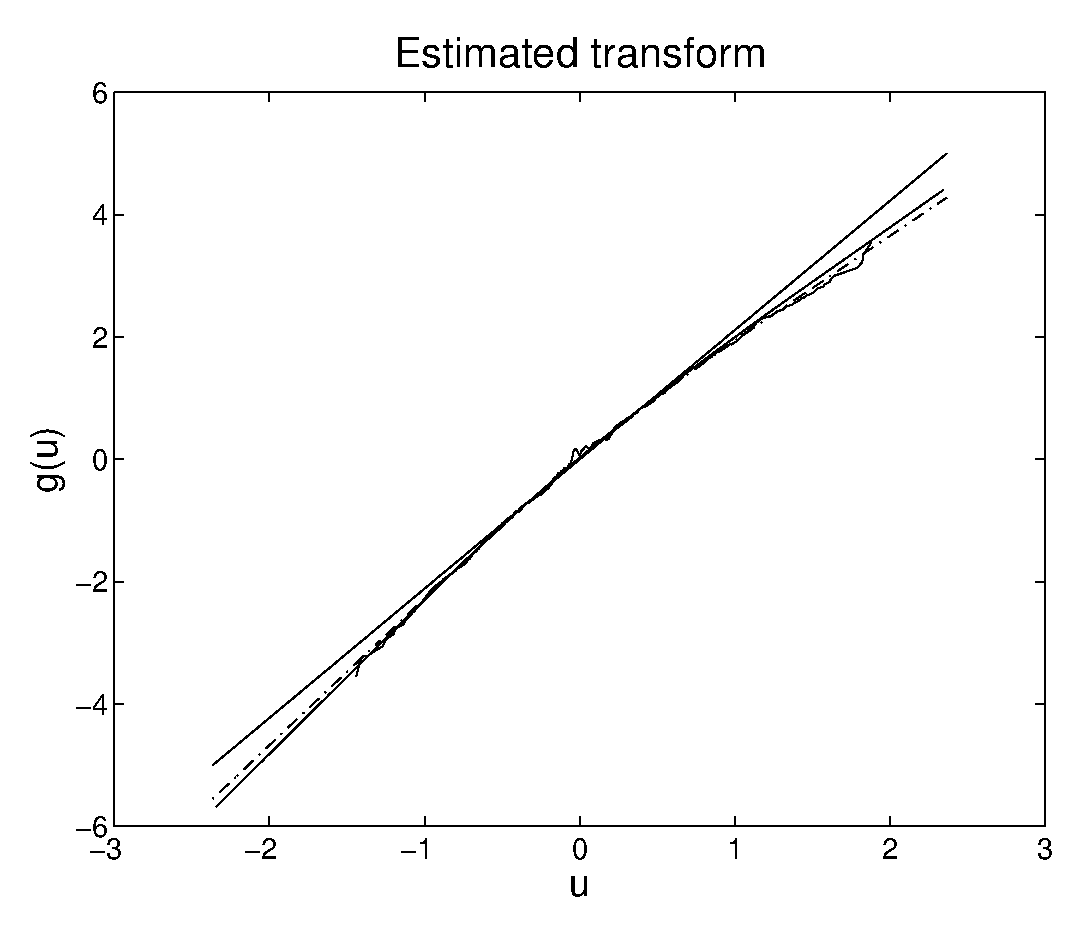
\includegraphics[width=\narrowfigwidth]{fig4grec}
\vspace{-3mm}
\caption[Transformation computed from reconstructed signal]{
The transformation computed from the reconstructed signal
{\tt y} (solid line) compared with
the transformation computed from the original signal {\tt xx}
(dashed dotted line).
}
\label{fig4-11}
\end{figure}

The value of the {\tt test} variable for the transformation
{\tt grec} is 0.84 and, as
expected, it is smaller than the value of {\tt test0} = 1.00 computed for the
transformation {\tt glc}. However, it is still significantly larger then the
values shown in Figure~\ref{fig2-3}, i.e.\ the signal {\tt y} is not
a Gaussian signal.

We turn now to estimation of the spectrum in the model from the simulated
data but first we transform data to obtain a sample $\tilde x(t)$:
{\small\begin{verbatim}
      L = 200
      x = dat2gaus(y,grec); %Gaussian process from reconstructed data
      SSx = dat2spec(x,L);  %Spectrum from Gaussian reconstructed process
\end{verbatim}}
\noindent
The important remark here is that the smoothing of the spectrum defined
by the parameter {\tt L}, see {\tt help dat2spec}, removes almost
all differences between the spectra in the three signals {\tt xx}, {\tt y},
and {\tt x}.
(The spectrum {\tt SSx} is normalized to have first spectral moment one
and has to be scaled down to have the same energy as the spectrum {\tt SS1} on page~\pageref{page:SS1}.)

Next, we shall simulate a random function equivalent to the reconstructed
measurements {\tt y}. The Nyquist frequency gives us the time sampling
of the simulated signal,
{\small\begin{verbatim}
      dt = spec2dt(Sx)
\end{verbatim}}\index[xcmds]{{\tt spec2dt}}
\noindent
and is equal to 0.25~seconds, since the data has been sampled with a
sampling frequency of 4~Hz. We then simulate 2~minutes
($2\times 60\times 4$ points) of the signal, to obtain a
synthetic wave equivalent to the reconstructed non-Gaussian
sea data.
{\small\begin{verbatim}
      Ny = fix(2*60/dt)  % = two minutes
      SSx.tr = grec;
      ysim = spec2sdat(SSx,Ny);
      waveplot(ysim,'-')
\end{verbatim}}
\noindent The result is shown in Figure~\ref{fig_2minutes}.
\end{rtex}

\begin{figure}
\centering
  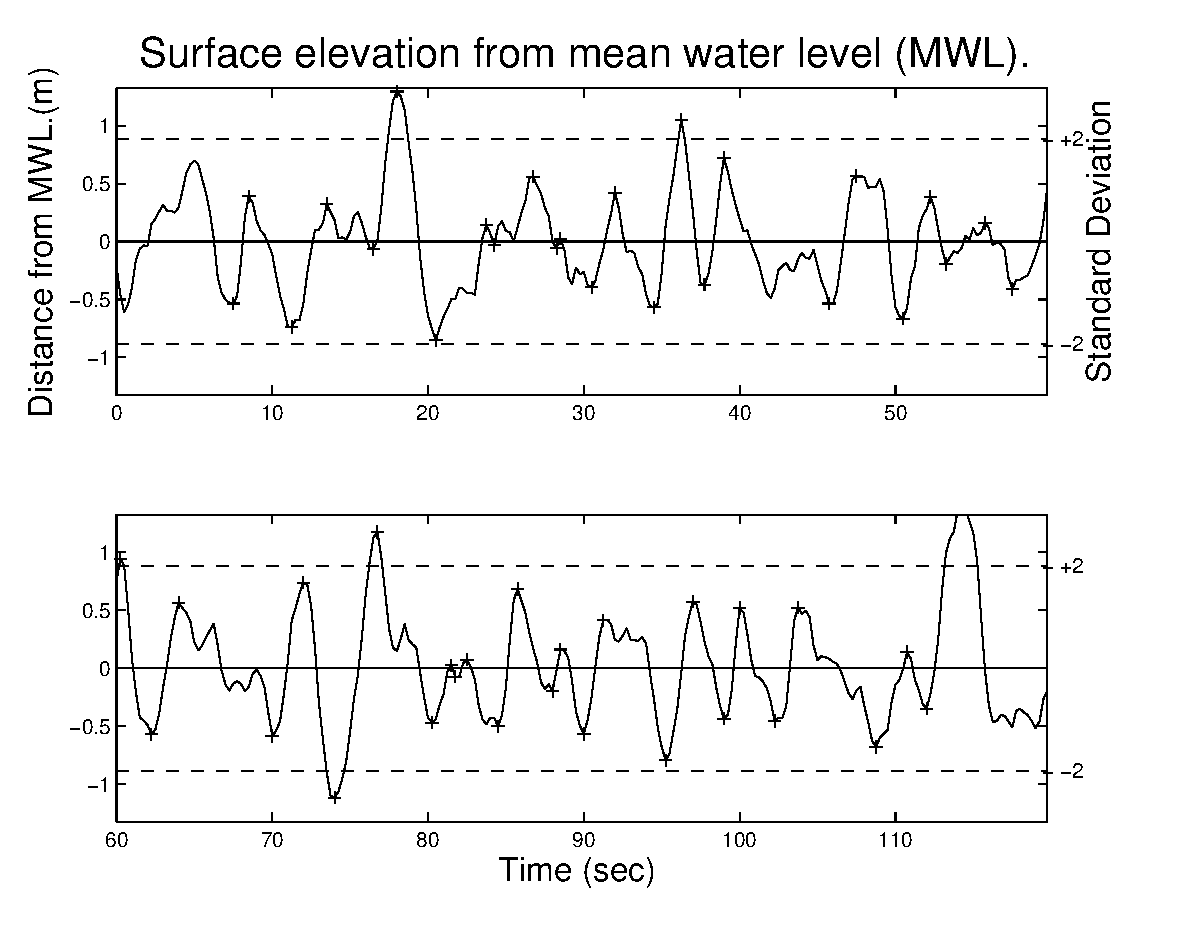
\includegraphics[width=\narrowfigwidth]{fig_2minutes}
\vspace{-3mm}
\caption[Two minutes of simulated sea data]{%
Two minutes of simulated sea data, equivalent to the
  reconstructed data.}
\label{fig_2minutes}
\end{figure}

In the next example we consider a signal with a given theoretical spectrum.
Here we have a problem whether the theoretical spectrum is valid for
the transformed Gaussian model, i.e.\ it is a spectrum $S(\omega)$ or is
it the spectrum of the linear sea $\widetilde S$. In the previous example
the spectrum of the transformed process was almost identical with the
normalized spectrum of the original signal. In
\cite{RychlikEtal1997Modelling} %Rychlik et al (1997)
it was observed that for sea data the spectrum estimated from
the original signal and that for the transformed one do not
differ significantly. Although more experiments should be done in order to
recommend using the same spectrum in the two cases,
here, if we wish to work with non-Gaussian models with
a specified transformation, we shall derive the $\widetilde S$ spectrum
by dividing the theoretical spectrum
by the square root of the first spectral moment of $S$.

\begin{cex}{Ex_sea_simulation}
Since the spectrum {\tt SS1} in Figure~\ref{fig2_spc}
is clearly two-peaked with peak frequency
$T_p = 1.1$ [Hz] we choose to use the Torsethaugen spectrum.
(This spectrum is derived for a specific location and we should not
expect that it will work well for our case.) The inputs to the programs are
$T_p$ and $H_s$, which we now compute.
{\small\begin{verbatim}
      Tp = 1.1;
      H0 = 4*sqrt(spec2mom(S1,1))
      ST = torsethaugen([0:0.01:5],[H0  2*pi/Tp]);
      plotspec(SS1), hold on
      plotspec(ST,[],'-.')
\end{verbatim}}
\noindent
In Figure~\ref{fig4-12}, we can see that the Torsethaugen spectrum
has too little energy on the swell peak. Despite this fact we shall use
this spectrum in the rest of the example.
\begin{figure}
\centering
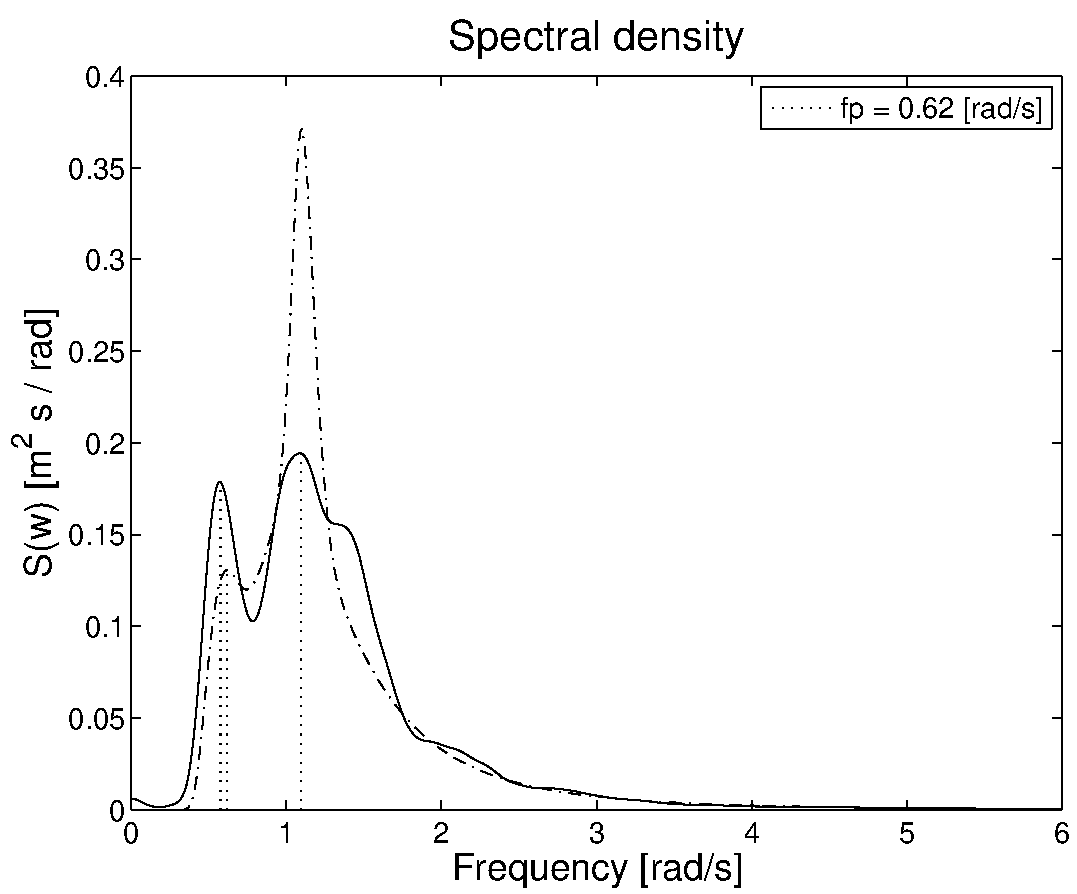
\includegraphics[width=\narrowfigwidth]{fig4spec}
\vspace{-3mm}
\caption[Comparison between spectra of
{\tt sea.dat}]{
Comparison between the estimated spectrum {\tt SS1} in the signal
{\tt sea.dat} (solid line) and the theoretical spectrum {\tt ST} of the
Torsethaugen type (dash-dotted line).
}
\label{fig4-12}
\end{figure}

We shall now create the spectrum $\tilde S(\omega)$ (= {\tt STnorm}),
i.e.\ the
spectrum for the standardized Gaussian process ${\widetilde X}(t)$ with
standard deviation equal to one.
{\small\begin{verbatim}
      STnorm = ST;
      STnorm.S = STnorm.S/sa^2;
      dt = spec2dt(STnorm)
\end{verbatim}}
The sampling interval {\tt dt} = 0.63 [s] (= $\pi / 5$),
is a consequence of our choice of
cut off frequency in the definition of the {\tt ST} spectrum.
This will however not affect our simulation, where any sampling interval
{\tt dt} can be used.

Next, we recompute the theoretical transformation {\tt gh}.
{\small\begin{verbatim}
      [Sk Su] = spec2skew(ST);
      sa = sqrt(spec2mom(ST,1));
      gh = hermitetr([],[sa sk ku me]);
      STnorm.tr = gh;
\end{verbatim}}

\noindent
The transformation is actually almost identical to {\tt gh} for
the spectrum {\tt SS1}, which can be seen in Figure~\ref{fig4_tr},
where it is compared to the Gaussian model {\tt g},
given by a straight line. We can see from the diagram that
the waves in a transformed Gaussian process $X(t)=G({\widetilde X}(t))$,
will have an excess of high crests and shallow troughs compared to
waves in the Gaussian process $\widetilde X(t)$. The difference is
largest for extreme waves with crests above 1.5~meters, where
the excess is 10~cm, ca~7~\%.
Such waves, which have crests above three standard deviations,
are quite rare and for moderate waves the difference is negligible.

In order to illustrate the difference in distribution for extreme waves
we will simulate a sample of 4~minutes of $X(t)$ with sampling
frequency 2~Hz. The result is put into \verb+ysim_t+.
In order to obtain the corresponding sample
path of the process $\widetilde X$ we use the transformation {\tt gh},
stored in {\tt STnorm.tr}, and put the result in \verb+xsim_t+.
{\small\begin{verbatim}
      dt = 0.5;
      ysim_t = spec2sdat(STnorm,240,dt);
      xsim_t = dat2gaus(ysim_t,STnorm.tr);
\end{verbatim}}
Since the process $\tilde X(t)$ always has variance one, in order to
compare the Gaussian and non-Gaussian models we scale
\verb+xsim_t+ %{\tt xsim$_t$}
to have the same second spectral moment as
\verb+ysim_t+,  %{\tt ysim$_t$},
which will be done by the following commands:
{\small\begin{verbatim}
      xsim_t(:,2) = sa*xsim_t(:,2);
      waveplot(xsim_t,ysim_t,5,1,sa,4.5,'r.','b')
\end{verbatim}}
\begin{figure}[t]
\centering
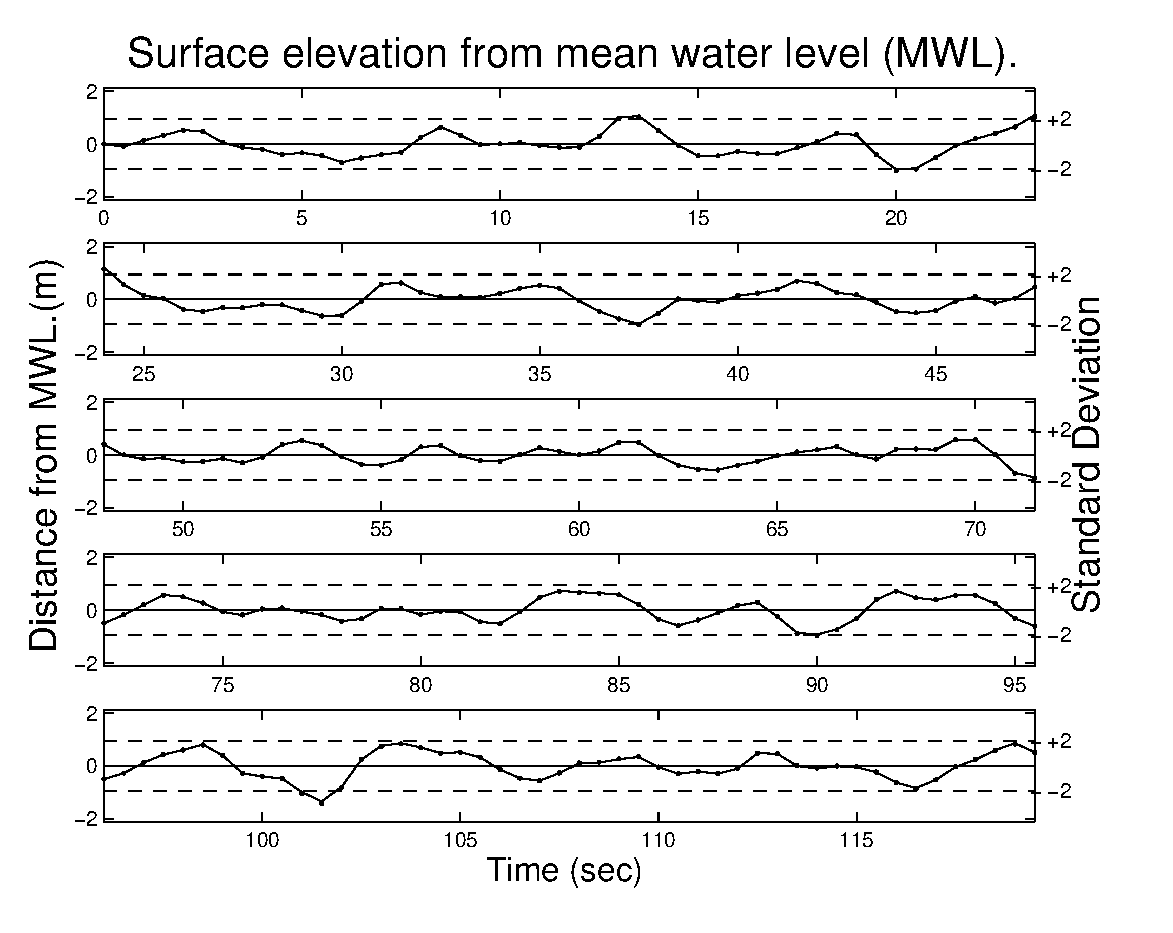
\includegraphics[width=\narrowfigwidth]{figure_sim1}
\vspace{-3mm}
  \caption[Gaussian simulated and transformed signals]{%
Simulated  $X(t)=G(\widetilde X(t))$ (solid line) compared
    with $\widetilde X(t)$ (dots) scaled to have the same $H_s$ as $X(t)$ for
    a theoretical
    spectrum  given by Torsethaugen spectrum {\tt St}.}
  \label{fig4-2}
\end{figure}

In Figure~\ref{fig4-2} we have waves that are not
extremely high and hence the difference between the two models is
hardly noticeable in this scale. Only in the second subplot we can see
that Gaussian waves (dots) have troughs deeper and crests lower than
the transformed Gaussian model (solid line). This also indicates
that the amplitude estimated from the transformed Gaussian and Gaussian
models are practically identical. Using the empirical transformation
{\tt glc} instead of the Hermite transformation
{\tt gh} would give errors of ca 11\%,
which for waves with higher significant wave height would give considerable
underestimation of the crest height of more extreme waves.
Even if the probability for observing an extreme wave during
the period of 20 minutes is small, it is not negligible for safety
analysis and therefore the choice of transformation is one of the most
important questions in wave modelling.

Since the difference between Gaussian and non-Gaussian model is not
so big we may ask whether 20 minutes of observation
of a transformed Gaussian process presented in this example is long enough
to reject the Gaussian model. Using the function {\tt testgaussian}
we can see that rejection of Gaussian model would occur very seldom.
Observe that the {\tt sea.dat} is 40 minutes long and that we
clearly rejected the Gaussian model.
\end{cex}


\index[xentr]{transformed Gaussian models|)}
\index[xentr]{transformed Gaussian models!simulation of|)}
\index[xentr]{simulation!of transformed Gaussian process|)}

\section{More on simulation  with \wf{}}\label{s:2.4}
The \wf{} toolbox contains additional routines for simulation of 
random loads and random waves. 
One important class used in fatigue analysis and in modelling
the long term variability of sea state are the Markov models, 
in which the model parameters are allowed to switch to new 
values according to a Markov chain.\index[xentr]{Markov!chain}
Another group of simulation routines generate non-linear waves and loads, 
like second order Stokes waves with interaction between 
frequency components in the Gaussian wave model, and 
Lagrange waves, with a horizontal deformation of  space. 
This  group includes a program to simulate the output of second
order oscillators with nonlinear spring,  when external force is
white noise. The nonlinear oscillators can be used to
model nonlinear responses of sea structures.

\subsection{Markov models}
The following routines from the {\tt simtools} module can be used to generate realistic 
load sequencies  for for reliability and fatigue analysis; see more in Chapter~\ref{cha:5}.
\begin{description}
\item[{\tt lc2sdat}] Simulates a load process with specified crossing spectrum and irregularity
\item[{\tt mcsim}] Simulates a finite Markov chain from its probability transition matrix
\item[{\tt mctpsim}] Simulates a Markov chain of turning points from transition matrix
\item[{\tt sarmasim}] Simulates an ARMA time series with Markov switching parameters
\item[{\tt smcsim}] Simulates a Markov chain with Markov switching regime
\end{description}

\begin{rtex}{SARMA}{Switching ARMA model}
In many applications, the standard stationary  time series Auto-regressive/Moving average ARMA-model, 
\cite[Ch.~7]{LindgrenRootzenSandsten2014}, can be made more realistic if the 
parameters are allowed to change with time, according to abrupt changes in environment conditions. 
Examples are found in econometrics \cite{Hamilton1989}, climate and environmental research \cite{AilliotMonbet2012}, automotive safety   \cite{Johannesson1998Rainflow}, and many other areas. 
A special case are the {\it Hidden Markov models} where the changes occur according to an 
(unobserved)  Markov chain

The \wf{} routine {\tt sarmasim} was developed by  Johannesson \cite{Johannesson1998Rainflow} 
in order to find a good model for stress loads on a truck serving on an irregular scheme, loading 
and unloading gravel. 
 The following example from {\tt sarmasim} illutrates the principles on an ARMA(4,2)-process swhitching
by a Markov {\it regime process} between two states.  \index[xentr]{Markov!hidden model}
\index[xcmds]{{\tt sarmasim}}
{\small\begin{verbatim}
    p1 = 0.005; p2=0.003;  % Switching probabilities
    P = [1-p1 p1; p2 1-p2];  % Markov transition matrix
    C = [1.00 1.63 0.65; 1.00 0.05 -0.88];  % MA-parameters 
    A = [1.00 -0.55 0.07 -0.26 -0.02; ... 
    		   1.00 -2.06 1.64 -0.98 0.41];  % AR-parameters
    m = [46.6; 7.4]*1e-3;  % Mean values for sub-processes
    s2 = [0.5; 2.2]*1e-3;  % Innovation variances
    [x,z] = sarmasim(C,A,m,s2,P,2000);  % Simulate 2000 steps
    plothmm(x,z)  % Ploting
    		   %  x = Switching ARMA, z = Markov regime process
\end{verbatim}}
Figure~\ref{fig:sarmasim} shows the hidden Markov states and the, seemingly non-stationary,  
ARMA-process. In fact, the Markov chain is simulated from its stationary distribution and each 
ARMA-section starts with the stationary distribution for that particular ARMA-process, so 
the process is stationary! 
\end{rtex}
\begin{figure}[tbh]
\centerline{
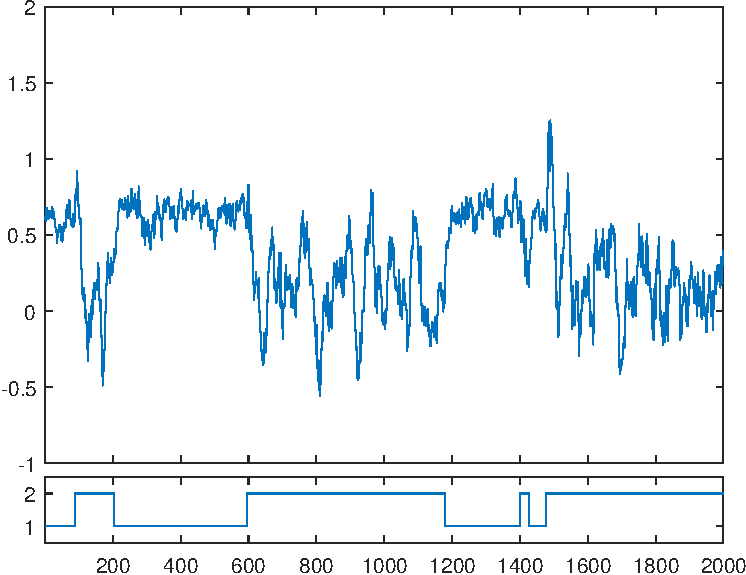
\includegraphics[width=\narrowfigwidth]{sarmasim}
}
\caption{Switching ARMA-process with Markov regime process.}
\label{fig:sarmasim}
\end{figure}


\subsection{Space-time and non-linear waves and loads}
The following routines in modules {\tt simtools} and {\tt lagrange} generate 
continuous time series and continuous space-time realizations. 
\begin{description}
\item[{\tt duffsim}] Generates a sample path of a 
linear or non-linear random oscillator \index[xcmds]{{\tt duffsim}}
\item[{\tt spec2wave} and {\tt spec2field}] Generate samples of space-time 
(transformed) \index[xcmds]{{\tt spec2field}}
 2D and 3D Gaussian waves  \index[xcmds]{{\tt spec2wave}}
\item[{\tt seamovie}] Makes a movie in time of 2D or 3D random waves
and optionally exports movie in {\tt avi} format  \index[xcmds]{{\tt seamovie}}
\item[{\tt seasim}] Old routine that generates a space-time Gaussian process and movie 
with 1D or 2D space parameter \index[xcmds]{{\tt seasim}}
\item[{\tt spec2ldat} and {\tt spec2ldat3D}] Routines in module {\tt lagrange} that generate 
front-back and crest-trough asymmetric \index[xcmds]{{\tt spec2ldat}}
modifications of Gaussian wave fields
\item[{\tt spec2nlsdat}] Simulates a random 2nd order \index[xcmds]{{\tt spec2nlsdat}}
non-linear wave from a spectral density
\end{description}

\begin{rtex}{Seamovieforexport}{How to export a sea movie}
In Section~\ref{ss:dirspec} we gave an example of how to use {\tt spec2field} 
to generate and plot a Gaussian sea surface with directional spreading. We now show how to 
use {\tt seamovie} to generate and save a movie of the time evolution of the sea. 

We define and plot the {\tt demospec} spectrum, with frequency independent 
spreading \index[xcmds]{{\tt demospec}}
{\small\begin{verbatim}
    SD = demospec('dir')
    plotspec(SD)
\end{verbatim}}
\noindent to get Figure~\ref{fig:demospec} and the structure
{\small\begin{verbatim}
SD = 
  struct with fields:
          S: [101 x 257 double]
        w: [257 x 1 double]
    theta: [101 x 1 double]
       tr: []
        h: Inf
     type: 'dir'
      phi: 0
     norm: 0
     note: 'Demospec: JONSWAP, Hm0 = 7, Tp = 11, gamma = 2.3853; Sprea...'
\end{verbatim}
}

\sidecaptionvpos{figure}{c}
%\begin{SCfigure}[0.75][t]
\begin{figure}[t]
\centerline{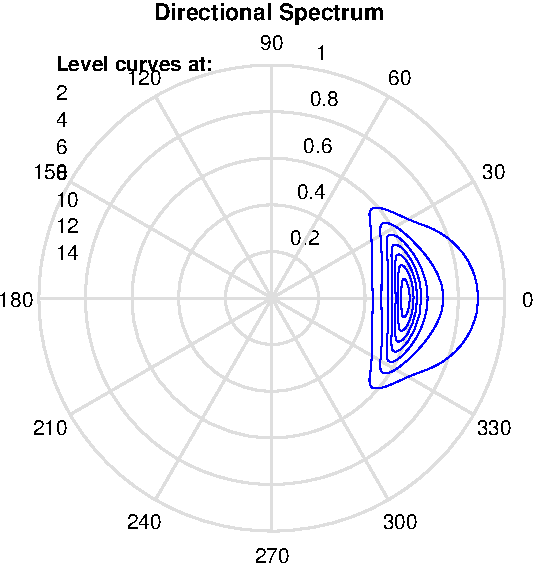
\includegraphics[width=0.5\textwidth]{fig_demospec}}
\caption[Directional spectrum {\tt demospec}]{Directional spectrum {\tt demospec}}
\label{fig:demospec}
%\end{SCfigure}
\end{figure}

To generate two minutes of a wave field of size 500[m] by 250[m] we define parameters 
by the function 
{\tt simoptset}\index[xcmds]{{\tt simoptset}}, 
generate the field with 
{\tt spec2field}\index[xcmds]{{\tt spec2field}}, 
and make three different types of movies with {\tt seamovie}\index[xcmds]{{\tt seamovie}}.  
{\small\begin{verbatim}
    opt = simoptset('Nt',600,'dt',0.2,'Nu',501','du',1,'Nv',251,'dv',1)
    rng('default')
    W = spec2field(SD,opt);  % structure with fields .Z, .x, .y, .t
    figure(2); Mv2 = seamovie(W,2); pause
    figure(3); Mv3 = seamovie(W,3); pause
    figure(1); Mv1 = seamovie(W,1,'sea.avi')
 \end{verbatim}}
\noindent The last movie command saves the movie as {\tt sea.avi} in the working directory. 
If {\tt sea.avi} already exists, the new movie file is given a random name. 
\end{rtex}

\begin{figure}
\centerline{
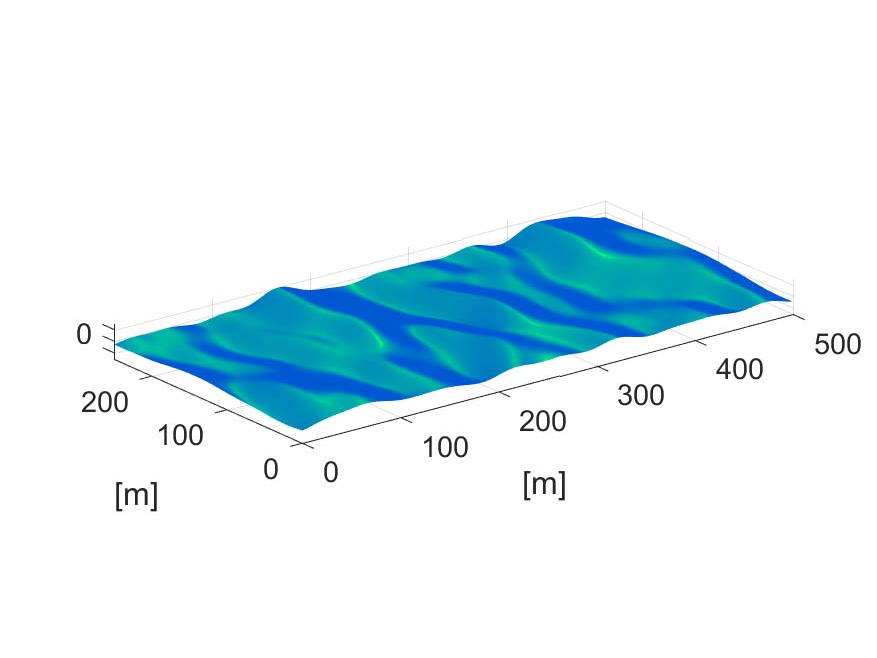
\includegraphics[width=130mm]{Mv1}
}
\vspace{3mm}
\centerline{
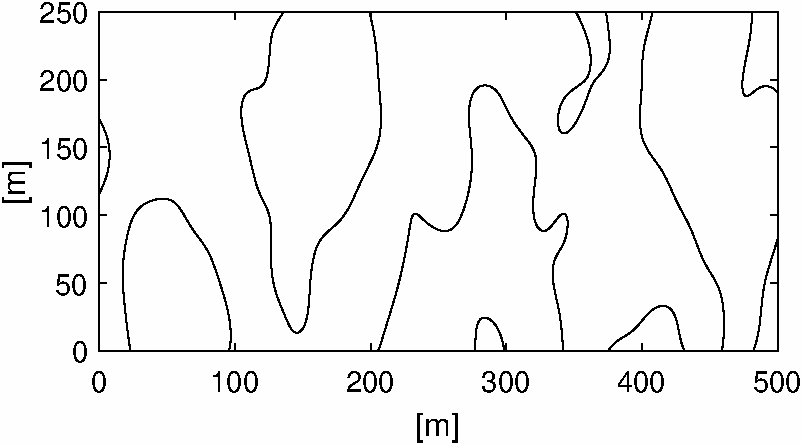
\includegraphics[width=130mm]{Mv2}
}\vspace{3mm}
\centerline{
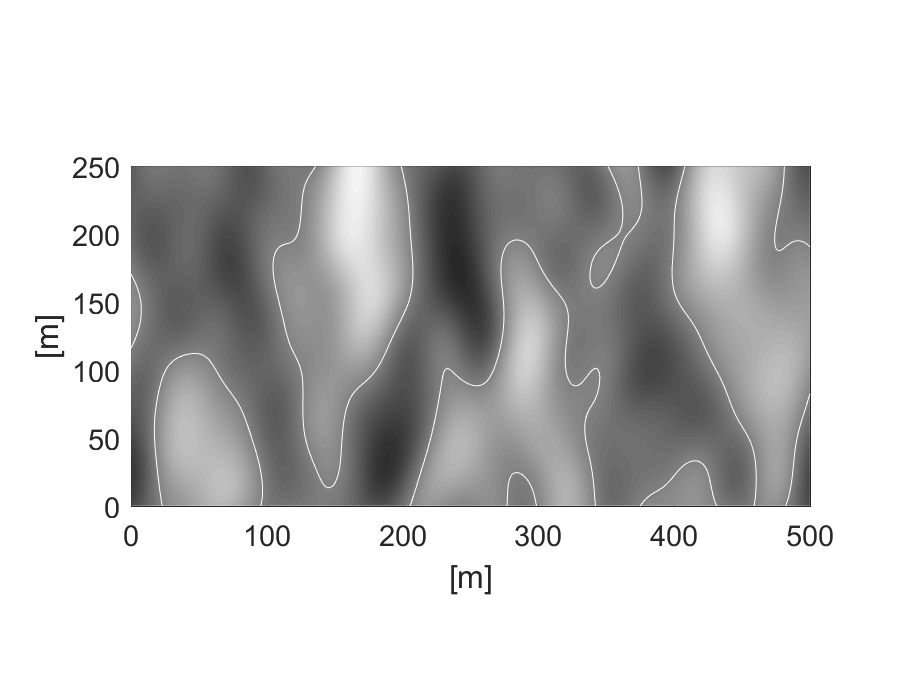
\includegraphics[width=130mm]{Mv3}
}
\vspace{-1mm}
\caption[Three aspects of Gaussian wave field]%
{Three aspects of a simulated Gaussian wave field with directional spectrum {\tt demospec('dir')}; last frames in 
{\tt Mv1}, {\tt Mv1}, and {\tt Mv3}.}
\label{Fig:threefields}
\end{figure}

\begin{remark}
The wave fields generated by {\tt spec2field} differ from animated wave fields used for example 
in feature films. They are intended to be used in applications where the fine structure, 
so important for the visual impression,  can be neglected. Examples involve extreme value analysis, 
fatigue loads, and ship dynamics.
\end{remark}

%\clearpage
\subsection{Structure of spectral simulation}
The following table explaines the sequencing of spectral simulation routines in modules {\tt simtools} and {\tt lagrange}. 
A (freq) or (dir) indicates the type of input spectrum.   
\vspace{5mm}

\begin{turn}{90}
\centering
\setlength\extrarowheight{3pt}
\begin{tabular}{||l|c|c|c|c||}\hline\hline 
\multicolumn{5}{||c||}{} \\
 \multicolumn{5}{||c||}{\raisebox{10pt}{\large \fo and \so order Gaussian waves in module {\tt simtools}}} \\ \hline
Routine & {\tt spec2sdat} & {\tt spec2wave} & {\tt spec2field} & {\tt spec2nlsdat}\\ \hline 
Type & \fo order Gaussian  & \fo order Gaussian  & \fo order Gaussian  & \so order Gauss-Euler \\
& time or space series & 2D space-time wave & 3D space-time field & 2D time wave \\
 & $\downarrow$ & $\downarrow$ & $\downarrow$ & $\downarrow$\\
Output & {\tt [x,xder]} & {\tt W.Z, .x, .t}& {\tt W.Z, .x, .y, .t} & {\tt [xs2,xs1]}\\
& & $\downarrow$ & $\downarrow$ & \\
Movie & & {\tt M = seamovie(W,type)} & {\tt M = seamovie(W,type)} &\\ \hline\hline 
\multicolumn{5}{||c||}{}  \\
 \multicolumn{5}{||c||}{\raisebox{10pt}{\large \fo and \so order Lagrange waves in module {\tt lagrange}}} \\ \hline
Routine & {\tt spec2ldat } (freq) & {\tt spec2lseries } (dir)  & {\tt spec2ldat3D } (dir)& {\tt spec2ldat3DM/P}\\ \hline 
Type & \fo order Lagrange 2D & \fo order Lagrange 2D & \fo order Lagrange 3D & \so order Lagrange 3D \\
& space/time components & time series & space/time components & space/time components\\
& $\downarrow$ & $\downarrow$ & $\downarrow$ & $\downarrow$\\
Output & {\tt [w,x]} & {\tt L.Z, .t, .points}& {\tt [w,x,y]}& {\tt [w,x,y,w2,x2,y2]}\\
& $\downarrow$ & $\downarrow$ & $\downarrow$ & $\downarrow$\\
Series/field & {\tt L = ldat2lwav} & \rule{7mm}{0.5mm}  & {\tt L = ldat2lwav3D} & {\tt L = ldat2lwav3D} \\
& $\downarrow$ & $\downarrow$ & $\downarrow$ & $\downarrow$\\
Movie &{\tt M = seamovie(L,type)} & {\tt M = seamovie(L,type)} & {\tt M = seamovie(L,type)} &{\tt M = seamovie(L,type)}\\ \hline\hline 
\end{tabular} 
\end{turn}
